\documentclass[11pt]{article}

\usepackage{natbib}
\bibliographystyle{abbrvnat}
\setcitestyle{authoryear,open={(},close={)}} 
\usepackage{multicol}
\usepackage{multirow}
\usepackage{booktabs}
\usepackage{caption}
\usepackage{amsmath}
\usepackage{longtable}
\usepackage{graphicx}
\usepackage{float}
\usepackage{bm}
\usepackage{graphics}
\usepackage{threeparttable}
\usepackage{amssymb}
\usepackage[margin=1in]{geometry}
\usepackage{setspace}
\usepackage{afterpage}
\doublespacing
\usepackage{subcaption}
\usepackage{subfig}
\usepackage{epigraph}
\usepackage{enumerate}
\usepackage{tabularx}
\usepackage{fancyhdr}
\usepackage{lscape}
\usepackage{mdframed}
\usepackage{mathtools}
\usepackage{array}
\usepackage{import}
\usepackage{fullpage}



\begin{document}
    \begin{titlepage}
    \title{A Case of Genetic Dilution in Improved Maize: Estimating Comparative Advantage of Adoption in Ethiopia}
% This second title is my preferred title at this point (28 Oct 2021). Open to other titles, but it shouldn't be longer than this one!

%     \author[1]{Oscar Barriga-Cabanillas}  
%     \author[2]{Cristina Chiarella}    
%     \author[2]{Juan Sebastian Correa}  	
%     \author[3]{Aleksandr Michuda}  

% 	\affil[1]{\small \emph{The World Bank}}
% 	\affil[2]{\small \emph{FAO}}
% 	\affil[3]{\small \emph{Assistant Research Professor at the Center for Data Science for Enterprise and Society, Cornell University}}
\author{%
 Aleksandr Michuda \footnote{Center for Data Science for Enterprise and Society, Cornell University}%
 \and Cristina Chiarella\footnote{UC Louvain}%
 \and Oscar Barriga-Cabanillas\footnote{The World Bank}%
  \and Juan Sebastian Correa \footnote{FAO}%
  }
%   Assistant Research Professor at the 
	\date{\today}

    \clearpage\maketitle
	\thispagestyle{empty}
	\vspace*{-2em}
    \begin{center}\begin{abstract}
			\noindent  
			Despite large investments in breeding and making high-yielding maize varieties available, evidence shows that few farmers consistently use them over time. We use an innovative methodology that studies the adoption trajectories of farmers over a three-round panel data set to explain low adoption rates with heterogeneous returns to adoption. By relying on self-reported use of improved seeds, we find that farmers do not adopt because they have a low comparative advantage and seemingly small to negative returns to adoption. To reconcile this result, we exploit unique information on maize DNA-fingerprinting collected over the same areas in 2018. We find that the negative returns to adoption mask heterogeneity driven by the variety of improved seeds used. Positive returns to adoption are found for those farmers that use higher-purity germplasm, drought-tolerant maize, and newly released varieties. Our findings point to the wide dispersion of older and genetically diluted varieties, for which poorer farmers are paying a premium. The implications of our findings speak to the need for policies to better target context and geography, expand accessibility of improved seeds, and make higher yields more inclusive.
			
			%Despite the large investments on creating better performing maize varieties, very few farmers consistently use them. We rely on four rounds of the ESS survey to answer this question. We find that relying on self reported use of hybrid seeds suggest there are negative returns to adoption. To reconcile this result, we use the information on genetic fingerprinting of seed available on the last ESS survey round to show that positive return for adoption appear only to exits for those farmers using seed with pure germoplast. We discuss the implications of our findings, showing that poorer farmers are the ones that consistently rely on second and third generation seeds, whose performance is debatable. 
        \end{abstract}\end{center}
        
        {\small \noindent\emph{JEL Classification}:
        	\emph{Keywords}: Improved maize, DNA-fingerprinting, Group Random Coefficient, Endogenous Switching Regression, Heterogeneous returns}

    \end{titlepage}
\maketitle
\newpage


%\begin{itemize}
%    \item Tim Weiss- hybrid subsidies
%    \item is there such a thing as traditional seeds?
%    \item Let's evaluate the effect of adoption in the context of Ethiopia
%    \item find ambiguous results, Why?
%    \item have access to DNA fingerprinting data
%    \item what do they say about adoption?
%    \item turns out that "adoption" isn't really a reliable concept/variable
%    \item most farmers are "adopting" under pretty conservative purity definitions
%    \item Let's see what happens with different varieties of seed, does adoption of that seed lead to positive yield effects?
%    \item can't use these methods but newer data has access to newer varieties where we're relatively more confident
%\end{itemize}

\section{Introduction}

%%% Why it is important
Food security is a major challenge in many East African countries, and Ethiopia is no exception, having historically struggled to provide an adequate and reliable food supply \citep{Ramakrishna2002-hv, Jaleta2018-oj}. Since the drought of 1984, Ethiopia has become increasingly reliant on maize, and as of today, maize constitutes the most widespread crop in the country.\footnote{FAO statistics show the total area cultivated with Maize in 2019 is 25\% larger than the next most widespread crop (sorghum), and 27\% and 139\% larger than the next two following crops, wheat and barley, respectively.} As Figure \ref{fig:maize_yields} shows, there is an upward trend in the total area cultivated with maize since 1990, with average yields almost doubling during this period. This increase in maize yields has also coincided with a dramatic decrease in undernourishment which has fallen from 47\% of the population in 2001 to 14\% in 2018 (The World Bank, 2021). Despite these positive gains, food insecurity still affects more than half the population of Ethiopia (ibid), reflecting that the progress achieved 
is not necessarily homogeneous across all subpopulations.\footnote{The country also has recently seen increases in food insecurity because of COVID-19, the conflict in Ethiopia’s Tigray region and the desert locust outbreak.}

\begin{figure}[htp]
    \centering
    \caption{Maize: Total area harvested and average yields} \label{fig:maize_yields}
    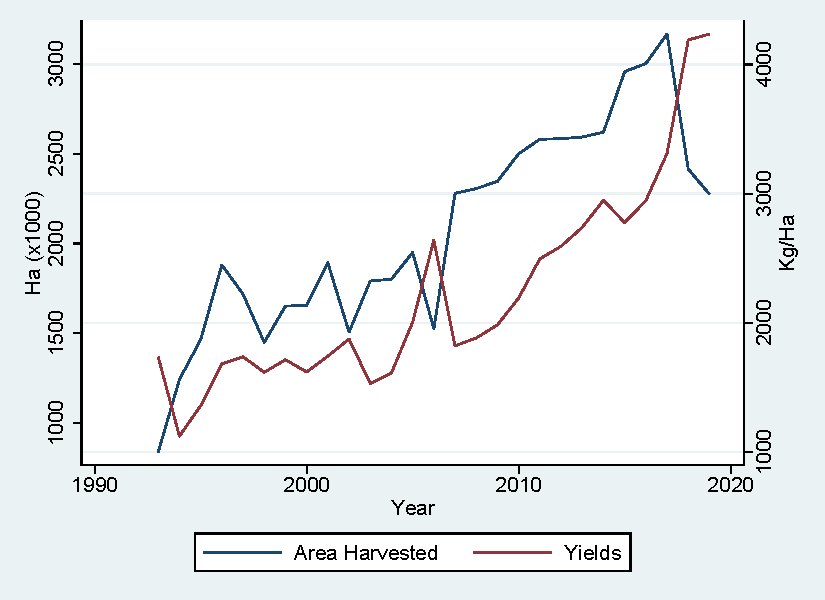
\includegraphics[width=.6\textwidth]{results/figures/Maize_yields.pdf}
    \vspace*{-1em}
    \begin{table}[H]
        \centering
        \begin{tabular}{p{0.6\textwidth}} 
            \begin{tablenotes}[flushleft]
                  \small
                  \item Source: Authors' calculations using FAOSTAT data 
                  \item Note: Yields are measured as the harvested production per ha for the area under cultivation
            \end{tablenotes}
        \end{tabular}
    \end{table}       
\end{figure}


%%%%% The puzzle 
The large disparities in yields and food security between the African continent and the rest of the developing world are often attributed to different adoption rates of green revolution technologies, such as improved seeds. Evidence has shown that the adoption of improved seed leads to increases in agricultural yields \citep{Carter2014-fm}, food security \citep{Shiferaw2014-op}, and poverty reduction \citep{Minten2008-tj}. Nevertheless, critics of green revolution technologies have also claimed that these technological packages have not been as profitable for many farmers in Africa as promised (with the exception of Ethiopia), given the high costs, and their heavy dependence on input subsidies \citep{Wise20}. \par
Even if the net returns to adoption of improved seeds are more conservative than often thought, the evidence regarding increased yields over traditional varieties is consistent across multiple contexts. Despite this evidence and numerous technological breakthroughs in maize germplasm with increased yields and drought tolerance, in the period between 2011 and 2015 only 13\% of maize farmers in Ethiopia have adopted improved seeds consistently, a large percentage has adopted new varieties inconsistently, and the lion share of farmers (62\%) have not used improved seeds at all during the same period. 

Several answers have been proposed to explain such low adoption of improved varieties. These include mainly the lack of liquidity and other economic constraints \citep{Carter2014-fm}, growing conditions such as the type of soil, input use, and farmer characteristics \citep{Munshi2004-og}, imperfections in credit markets \citep{Croppenstedt2003-pq}, ambiguously defined property rights \citep{Place2000-el}, lack of commitment devices \cite{Duflo2009-iv}, high transportation costs that increase the cost of agricultural inputs \citep{Byerlee2013-qk}, and improved seed supply constraints \citep{Bird2020-nt}. In this context, there is still a large percentage of the population not using improved seed varieties, or using varieties that are over 20 years old. With such old seed, there is evidence that yield improvement and disease resistance in these seeds are waning\citep{Abate2015-rj}. The variety of these constraints and their dispersion across subpopulations and locations speaks to considerable heterogeneous returns to adoption.      

%%%% Let's evaluate the effect of adoption in the context of Ethiopia

In this paper, we revisit the mechanism proposed by \citep{Suri2011-oi}, where a lack of adoption of improved seed varieties is the result of farmers' heterogeneous returns to the new technology. Ignoring such heterogeneity can hide the true impact of adoption, as different sub-populations' returns may be impacted by the same technology in different, and even opposite ways, despite it providing high average returns. The heterogeneous returns to adoption are modeled as a farmer's unobservable comparative advantage using a Correlated Random Coefficient (CRC) model. In the original paper, \citep{Suri2011-oi} finds that farmers’ lack of adoption is driven by insufficient net benefits to the technology stemming from poor infrastructure that increase the cost of access. Similar work in Ethiopia on improved chickpea varieties suggests that the economic returns to adoption plays a major role in the decision to adopt \citep{Michler2018-wk}. 

%% Expand a bit on the methods
We build on this literature by investigating hybrid maize seed adoption in Ethiopia, focusing on how heterogeneous returns drive the decision to use improved seed varieties. We implement two complementary estimation strategies. First, we implement a Group Random Coefficients estimation, which builds on \cite{Suri2011-oi} in \cite{Tjernstrom_Emilia_Dalia_Ghanem_Oscar_Barriga_Cabanillas_Travis_J_Lybbert_Jeffrey_D_Michler_and_Aleksandr_Michuda2020-bc} using a General Method of Moments (GMM) Estimator that allows us to test the assumptions assumed by \cite{Suri2011-oi}, as well as provide more economically interpretable results. The advantage of our estimation strategy is that we do not rely on identification from a valid instrument, but a strategy similar to \cite{Chamberlain1984-uk}. For this strategy, we rely on the first three survey rounds of the Ethiopian Socioeconomic Survey (ESS), panel dataset that allows us to follow the same households across time (from 2011 to 2015). Using self-reported information on the seed variety (improved or traditional), we compare the adoption trajectories over three rounds. The results show that the returns to adoption are in most cases, not statistically significant, and only significant with wave 3 adoption. This posits a puzzle that motivates our next estimation strategy.

We expand our results using the fourth round of the ESS (conducted in 2018), which provides a unique opportunity to understand why improved seed varieties seem not to increase returns when adopted. The ESS4 collected DNA fingerprints of harvested cropcuts in selected plots and compared its genetic material with a reference library of available varieties in Ethiopia. This provides critical information not only about the seed types but also about their purity, sources, and their year of release. We exploit this uniquely rich information to compare different definitions of improved seeds. Specifically, we compare the returns to the self-reported use of new, second generation or recycled varieties, with those of improved seeds as defined by their genetic material, comparing different purity thresholds (or degrees of no-contamination with other varieties), year of release, types of varieties, and their sources. Because the latest survey round is not a continuation of the first three rounds, our second estimation strategy implements an Endogenous Switching Regression (ESR) approach, a standard estimation strategy to study the question of adoption with cross-sectional data (\citealt{Marenya2020-kb}, \citealt{Shiferaw2014-op}), given its capacity to account for unobserved heterogeneity in adoption. 

The results of the ESR find negative effects of adopting improved seeds, as per farmer self-reports. But the comparison of the different improved seed definitions using the DNA fingerprinting sheds light on possible explanations for this apparent puzzle. We find that when the definition of improved seed is based on greater purity of the germplasm (95\% of purity or more), the returns to adoption for those that used such improved varieties becomes positive and significant. We obtain similar results when evaluating the specific effects of adopting drought-tolerant maize varieties, CGIAR or Exotic varieties, or more recently released varieties.


Taken together, the negative and not statistically significant returns to adoption we find from both estimation strategies reflect the loose definition of improved seeds when such improved varieties are self-reported by farmers. Only a subset of farmers use the purest genetic varieties, drought-tolerant varieties, or newly released varieties, which tend to provide higher returns. This implies that poorer farmers are paying a premium for genetically diluted hybrids, which has far-reaching policy implications about the need to foster a more inclusive policy when making the best performing seeds available to all farmers.


Our results contribute to the literature on the drivers of low adoption rates. The consensus in this literature is that the success of improved varieties depends on a range of factors, and that the widespread adoption of  improved seeds is the result of complementary conditions and inputs that allow farmers to extract the full potential of these varieties. Specifically, extension services and on-farm field trials, seed variety characteristics and rainfall have been found to be crucial to the adoption of improved maize in Tanzania \citep{Kaliba2000-jh}. In the specific case of Ethiopia, labor, fertilizer use, farmers’ experience with extension packages, rainfall suitability and prices have been shown to increase the opportunity cost of not adopting improved wheat varieties \citep{Wale2006-bv}. Market access and the accessibility of extension services are also critical in the adoption of improved chickpea varieties in Ethiopia \citep{Verkaart2019-ol}. Other important determinants of heterogeneous effects include risk aversion \citep{Holden2016-vy}, farm size \citep{Ghimire2015-bd}, and credit constraints \citep{Simtowe2008-jn,Balana2020-hx}. 


% A different branch of the literature provides an alternative explanation for the low adoption rates, focusing on heterogeneous potential returns to adoption \citep{Suri2011-oi}. This literature suggests that even if returns to adoption are high, farmers may fail to adopt if they face low comparative advantage to adoption. Other methods used in the literature fail to account for this heterogeneity, admitting only the presence of time-constant and/or time-varying unobserved heterogeneities (depending on the data structure) for identification purposes \citep{Kassie2018-xn,Falco2011-rt}. 

We contribute to this literature by exploring heterogeneous comparative advantages to adoption in Ethiopia between 2011 to 2015, controlling for important drivers of adoption such as rainfall (found to be the main driver of heterogeneous effects for adopting agronomic packages \citealt{Marenya2020-kb}, \citealt{Katengeza2019-af}), labor and input use. Our paper also provides a novel way of visualizing GRC results, which become difficult to interpret with longer time variables. Our findings also provide an alternative hypothesis to the low-returns to adoption, namely that the wide dispersion of older generations and recycled improved seeds, which may be both resulting in lower yields and altering farmers' input use in response to a mis-classified seed. This also implies a methodological discovery when investigating hybrid seed adoption: the absence of a true control group to use for analysis. With more time and more genetic dilution, it becomes more and more likely that even those that do report hybrid use are still likely using some level of hybrid.

The article continues as follows. In Section \ref{sec:data}, we describe the data used, the sample frame, general farmer and farm characteristics, and improved seed adoption levels. Section \ref{sec:strategy} presents the methodological details of our two estimation strategies. Section \ref{sec:results} shows the estimations results, and Section \ref{sec:conclusion} presents the conclusion and implications of our analysis.


\section{Data}\label{sec:data}

This study uses the Ethiopia Socioeconomic Survey (ESS), part of the Agricultural Sample Survey (AgSS), a nationally representative survey designed to collect agricultural information for the major crops in Ethiopia. The survey is a joint effort of the the Central Statistics Agency of Ethiopia, the World Bank and CGIAR (Consortium of International Agricultural Research Centers) \citep{kosmowski2020shining}. The ESS contains four survey modules designed to obtain specific information about the different stages in the agricultural season. A post-planting questionnaire obtains information about the parcel, crop roster, seed roster and input use. A post-harvest questionnaire collects information about crop harvests by parcel (which includes cropcut measurements for selected plots), and crop disposition. These two instruments are complemented with a household and a community questionnaire, which obtain information on household characteristics, labor, land, expenditure, and community characteristics such as market prices and economic activities, respectively.

\subsection{The Three Round Panel}

There were significant differences between the analysis carried out in ESS 1-3 and the most recent, ESS4. Most notably, the ESS4 is no longer a panel dataset made up of the households of ESS 1-3, but it includes important information on the DNA fingerprinting of seed type, which can be used to calculate misclassification rates. This is important information as the first three waves of ESS only included self-reported hybrid maize status. Since our estimation strategy requires a balanced panel dataset of maize growers, our main analysis includes the first three waves of the ESS. We use the fourth wave for validation, and to explore the impact of specific types of improved seeds.

Figure \ref{map:regions} shows the spatial distribution of the locations of the households in the study. These are households that grow either improved or conventional maize and that are observed for the three rounds of the survey. Most households come from the northwest region of Amhara, Tigray and Oromiya which is consistent with where maize is mostly grown in Ethiopia \citep{Abate2015-rj}.

\begin{figure}[H]
    \centering
    \caption{Spatial Distribution of Households Surveyed}\label{map:regions}
    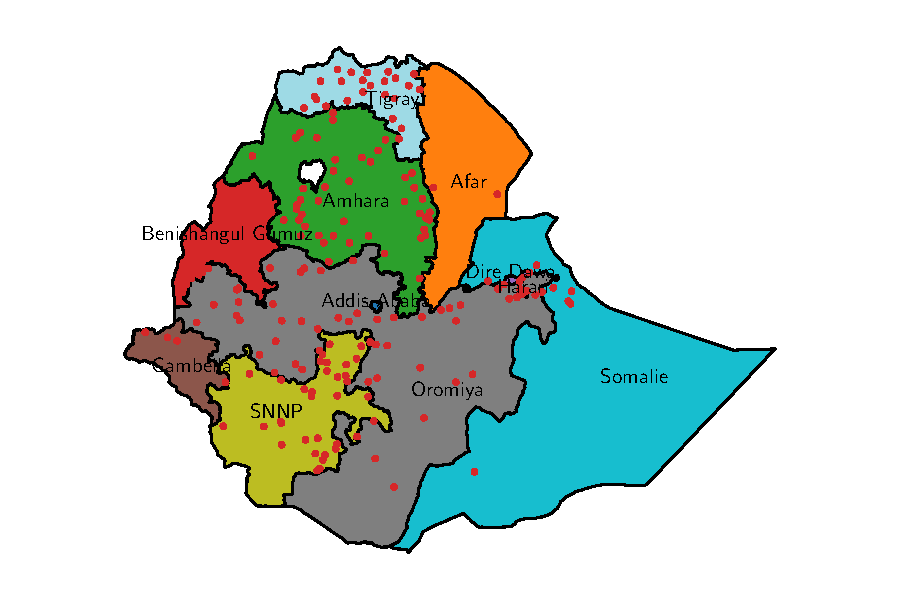
\includegraphics[width=.7\textwidth]{results/figures/map_hhids.pdf}
    \vspace*{-1em}
    \begin{table}[H]
        \centering
        \begin{tabular}{p{0.6\textwidth}} 
            \begin{tablenotes}
                  \small
                  \item Note: Red markers denote the locations of households
            \end{tablenotes}
        \end{tabular}
    \end{table}  
\end{figure}

Table \ref{tbl:summary} shows a set of summary statistics for the sample. The mean parcel size for a household is about 0.15 Ha, with a maximum size of a little less than 1.5 Ha. Harvest labor is disproportionately skewed to family participation with around 20 days of harvest labor being conducted by family members and only about 2 days for hired labor. This is indicative of either malfunctioning labor markets, income constraints or high supervision costs. The distances to some key areas are also highlighted in Table \ref{tbl:summary}. On average, households are around 13 kilometers away from an asphalt road and almost 60 kilometers away from the nearest market. This makes both the purchase of improved seed and the marketing of yields subject to transportation costs and a difficult enterprise. Fertilizer costs are on average 8,350 Birr ($\thicksim$178 USD), with a large amount of the sample not using fertilizer at all. This is particularly important in the context of improved maize seed use as it requires fertilizer to be most effective. Only 5\% of the sample irrigates their crops making households susceptible to weather shocks.


\afterpage{{\footnotesize\tabcolsep=1pt  % hold it local
    \begin{table}
\centering
\caption{Summary Statistics for Households}
\label{tbl:summary}
\begin{tabular}{lllll}
\toprule
                             & Wave &       1.0 &       2.0 &       3.0 \\
\midrule
Parcel Size & N &  1,116.00 &  1,116.00 &  1,116.00 \\
                             & Mean &      0.31 &      0.32 &      0.30 \\
                             & Std. Dev. &      0.36 &      0.39 &      0.35 \\
Household Labor for Harvest (Days) & N &  1,116.00 &  1,116.00 &  1,116.00 \\
                             & Mean &     45.51 &     38.29 &     36.33 \\
                             & Std. Dev. &     71.11 &     54.58 &     46.56 \\
Hired Labor for Harvest (Days) & N &  1,116.00 &  1,116.00 &  1,116.00 \\
                             & Mean &      4.27 &      3.38 &      4.89 \\
                             & Std. Dev. &     25.93 &     17.08 &     54.11 \\
Age of Household Head & N &  1,106.00 &  1,086.00 &  1,102.00 \\
                             & Mean &     43.85 &     45.91 &     48.23 \\
                             & Std. Dev. &     14.31 &     14.17 &     14.33 \\
Sex of Household Head & N &  1,109.00 &  1,114.00 &  1,108.00 \\
                             & Mean &      1.15 &      1.15 &      1.16 \\
                             & Std. Dev. &      0.36 &      0.36 &      0.36 \\
Years of Education of Household Head & N &  1,106.00 &  1,085.00 &  1,102.00 \\
                             & Mean &      1.46 &      1.56 &      1.64 \\
                             & Std. Dev. &      2.71 &      2.77 &      2.92 \\
Total Rainfall (mm) & N &  1,113.00 &  1,088.00 &  1,106.00 \\
                             & Mean &    899.23 &    953.98 &    943.03 \\
                             & Std. Dev. &    240.43 &    237.46 &    267.07 \\
Does Household have Title to land? & N &  1,113.00 &  1,088.00 &  1,106.00 \\
                             & Mean &      0.43 &      0.52 &      0.61 \\
                             & Std. Dev. &      0.50 &      0.50 &      0.49 \\
Crop Cut Dry Yield (kg/ha) & N &  1,105.00 &  1,103.00 &  1,103.00 \\
                             & Mean &     86.51 &    251.69 &    438.42 \\
                             & Std. Dev. &    200.25 &    532.17 &    786.49 \\
Self-reported Yields (kg/ha) & N &  1,043.00 &  1,075.00 &  1,064.00 \\
                             & Mean &    187.18 &  1,314.04 &  1,224.65 \\
                             & Std. Dev. &    435.03 &  1,157.66 &  1,105.53 \\
\bottomrule
\multicolumn{6}{l}{Note: Parcel size, yield and distance variables winsorized at the 1\% level.}
\end{tabular}
\end{table}

    \vspace*{-4em}
    \begin{table}[H]
        \centering
        \begin{tabular}{p{0.7\textwidth}} 
            \begin{tablenotes}
                  \small
                  \item Note: Author's calculations using ESS. Maize farmers only.
            \end{tablenotes}
        \end{tabular}
    \end{table}  
    \newpage
}}

The ESS has both self-reported and crop cut yields available. This provides two sources of yield information, although self-reported yields seem to be overly large compared to either fresh or dried crop cut yields. Self-reported yields are both more susceptible to behavioral biases, but also to confusion caused by differences in assumed units. In general, though, the sample with available cropcut yields cuts down the available sample significantly, given that cropcuts were only collected for a subsample of randomly selected households, which limits their power.


\subsection{Improved seeds}

A crop seed is considered “improved” in Ethiopia if it was tested by breeders and evaluated to be superior to existing varieties  (\citep{MoA13}; \citep{kosmowski2020shining}). In Ethiopia, the government controls most of the seed system, with local agricultural offices or extension agents assessing the demands of different varieties. The MoA decides the seed quantities to be produced, and actors such as regional seed enterprises, seed companies, seed unions, are involved in the production of certified seeds, that are primarily distributed by seed producer cooperatives (SPCs), which account for 37\% of the total distribution in the country (\citep{kosmowski2020shining}). An improved seed can be obtained directly from such distribution centers (which would distribute a first generation seed), or it could be cultivated from second or later generations from the originally bred seed. In the survey, farmers are asked to report whether the variety they used was a first-generation improved seed, second generation, recycled, or a traditional variety. When buying seeds, farmers might be able to identify the variety they are looking for, but it is unlikely that they would be aware of the source. 

Fifty four varieties have been released in Ethiopia since 1990, out of which seven were released between 1990 to 1999, 29 between 2000 to 2009, and 18 between 2010 to 2019. Thirty four such varieties contain International Maize and Wheat Improvement Center (CIMMYT) germplasm, out of which, 10 Drought-tolerant maize varieties (DTMZ) and 8 Quality protein maize (QPM) were released (most of these between 2010 to 2019). Out of the CIMMYT-related germplasm, ten are open-pollinated varieties (OPVs) and 25 are hybrid (\citep{kosmowski2020shining}).

The fourth wave of the ESS introduced DNA fingerprinting of barley, maize, and sorghum for the first time. The collection of cropcuts for crop yield estimation facilitated the process for DNA fingerprinting. For the cropcuts, a 4 square meter quadrant was randomly selected in each plot, and total production harvested from the quadrant was weighed (both when freshly harvested and when dried). The DNA material was extracted from samples from the dried cropcuts, and were then matched with the genetic material of the maize DNA reference library for Ethiopia, obtained from a CIMMYT and Ethiopian Institute of Agricultural Research (EIAR) project. The collection of DNA samples focused on eight regions. In each enumeration area (EA) of these regions, a random sample of plots was selected, with a maximum of 10 fields for each crop. As a result, 505 plots were selected for DNA fingerprinting, corresponding to 447 households. 

The DNA fingerprinting process matched the genetic material of each sampled harvest with that of the reference library. The resulting matching process returns the name of the crop variety matched, its germplasm origin or their pedigree (whether they are a CIMMYT line, EIAR,  International Institute of Tropical Agriculture (IITA) or private), the breeder or maintainer, and the year of their release (which could be indicative of the number of generations a seed had been cultivated), as well as the genetic purity of the sample (the degree of non-contamination with other genetic varieties). It also informs whether the harvested seeds are open-pollinated varieties (OPVs) or hybrids; drought-tolerant maize varieties (DMTZ) or quality protein maize (QPM). This rich information about seed varieties provides a unique opportunity to further understand impacts differentiated by type of seed, degree of purity, year of release or source. Figure \ref{fig:adoption_r4} shows adoption rates in the fourth round for improved varieties, using the above characteristics as different definitions.

We find that 38\% of households self-report adopting a “new” improved variety (SR2 in Figure \ref{fig:adoption_r4}), and 43\% report adopting a “new”, “second generation” or “recycled” improved variety (SR1). Considering a household as adopter if the household planted an improved variety in at least one of their plots, leads to classifying all households where a DNA sample was obtained as users of improved seed variety, a result that holds when the purity threshold of 70\% (DNA 70) is used. It is only when using purity thresholds of 90 and 95\% (DNA 90, DNA 95 in Figure \ref{fig:adoption_r4}, respectively), that adoption rates of improved varieties change to 91 and 54\% of sampled households, respectively. We also find that 62\% of households adopted a hybrid variety, compared to 38\% that adopted an open-pollinated variety, and 15\% of households adopted a drought-tolerant maize variety, while 63\% of households that adopted an improved variety use a CGIAR-derived germplasm, and 79\% use an exotic germplasm. Finally, 64\% of households adopted a variety that was released in the year 2000 or after, and 24\% adopted a variety that was adopted in the year 2010 or after.

\begin{figure}[htpb]
    \centering
    \caption{Adoption rates of improved varieties in 2018 (by self-report, purity level, crop type, source and year of release)}\label{fig:adoption_r4}
    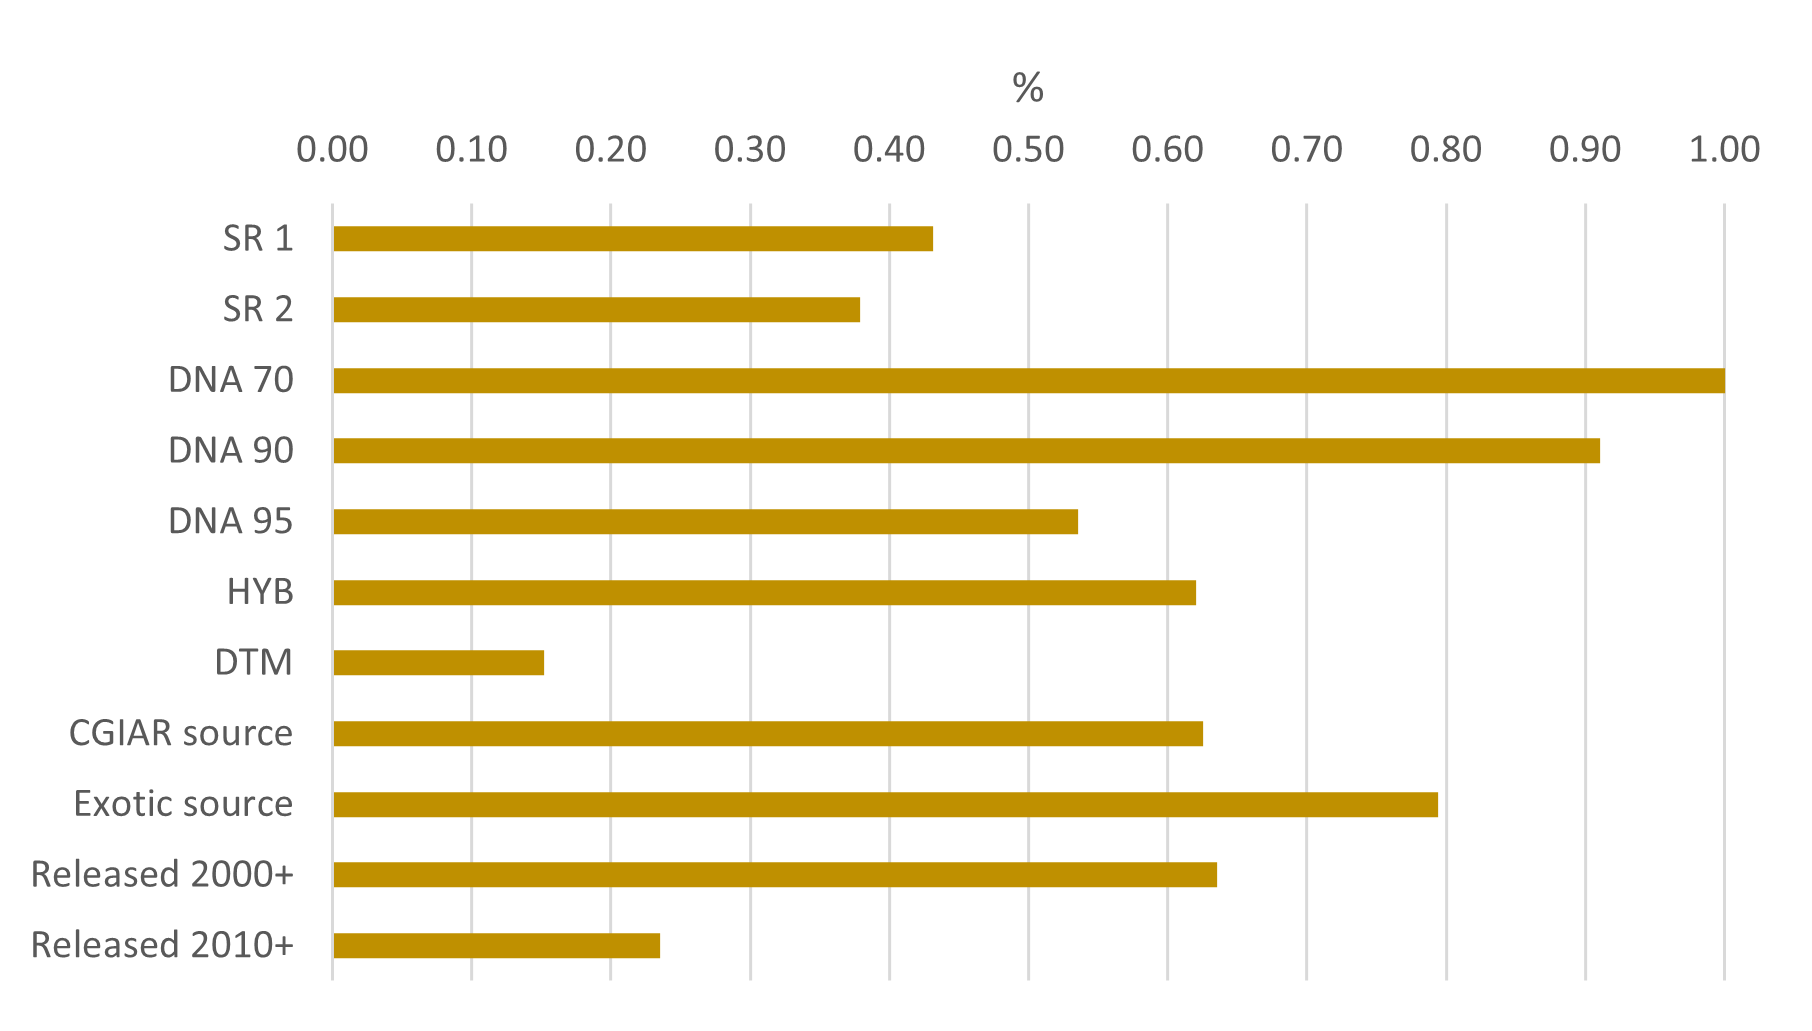
\includegraphics[width=.7\textwidth]{results/figures/adoption_r4.png}
    \begin{table}[H]
    \centering
        \begin{tabular}{p{0.7\textwidth}} 
            \begin{tablenotes}
                  \small
                  \item Note: Shares represent the proportion of adopters among maize farmers. Acronyms include: SR1 [=1 if New, 2nd gen or recycled, =0 if Traditional]; SR2  [=1 if New, =0 if 2nd gen, recycled or traditional]; DNA70 - Improved if purity $>=$70$\%$; DNA90 - Improved if purity $>=$90$\%$; DNA95 - Improved if purity $>=$95$\%$; HYB - Improved DNA, [=1 Hybrid, 0=Open pollinated]; DTM - Drought tolerant Maize [=1 DTM, 0=otherwise], CGIAR source [=1 if germplasm associated to a CGIAR-related thread], Exotic source [=1 if germplasm associated to an exotic source], Released 2000+ [=1 if DNA associated to a variety released on year 2000 or later], Released 2010+ [=1 if DNA associated to a variety released on year 2010 or later]. QPM is not included as there are too few households planting QPM seeds (n=6).
            \end{tablenotes}
        \end{tabular}
    \end{table}   
\end{figure}

These ratios are in line with prior findings. In the regions of Oromia, Amhara, Tigray, and SNNPR, adoption rates of improved maize varieties of 39\% of households were found, according to self-reported information (\cite{Zeng15}). In the regions of Amhara, Benishangul-Gumuz, Oromia, SNNPR, and Tigray, adoption rates of improved maize varieties were found for 27\% of households (\cite{Jaleta2018-oj}). In Oromia, SNNPR, and Benishangul-Gumuz adoption of improved varieties per farmers’ self-reports was found for 84\% of maize growers in 2011, and 88\% of maize growers in 2013 (\cite{Yirga17}).

Understanding the effects of improved seed adoption is not only challenging because there could be multiple ways of establishing what constitutes an improved seed, but also because such definitions may or may not overlap, or because farmers may also misclassify a variety as improved. Figure \ref{fig:missclassification} shows the correlation between the different definitions discussed above. For those seeds for which genetic material was obtained, the correlation with the self-reported seeds indicator is low, especially when using lower purity cutoff thresholds. 

\begin{figure}[htpb]
    \centering
    \caption{Correlation of different definitions of improved seeds, 4th round}\label{fig:missclassification}
    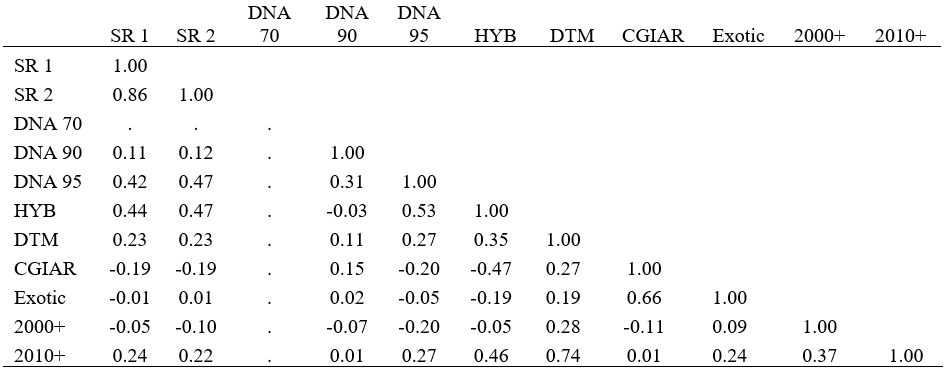
\includegraphics[width = 0.9\textwidth]{results/figures/missclassification.png}
    \vspace*{-2em}
    \begin{table}[H]
        \centering
        \begin{tabular}{p{1\textwidth}} 
            \begin{tablenotes}
                  \small
                  \item Note: Shares represent the proportion of adopters among maize farmers. Acronyms include: SR1 [=1 if New, 2nd gen or recycled, =0 if Traditional]; SR2  [=1 if New, =0 if 2nd gen, recycled or traditional]; DNA70 - Improved if purity $>=$70$\%$; DNA90 - Improved if purity $>=$90$\%$; DNA95 - Improved if purity $>=$95$\%$; HYB - Improved DNA, [=1 Hybrid, 0=Open pollinated]; DTM - Drought tolerant Maize [=1 DTM, 0=otherwise], CGIAR source [=1 if germplasm associated to a CGIAR-related thread], Exotic source [=1 if germplasm associated to an exotic source], Released 2000+ [=1 if DNA associated to a variety released on year 2000 or later], Released 2010+ [=1 if DNA associated to a variety released on year 2010 or later]. QPM is not included as there are too few households planting QPM seeds (n=6).
            \end{tablenotes}
        \end{tabular}
    \end{table}       
    
\end{figure}

\section{Estimation Strategy}\label{sec:strategy}

\subsection{Group Random Coefficient Model}

Since ESS1-ESS3 do no have DNA fingerprinting, we are left with only self-reports of hybrid use. We use these variables in a Group Random Coefficiens (GRC) approach to investigate the heterogeneous effects of adoption. The advantage of the GRC approach is that we do not rely on identification from a valid instrument, but on modelling the heterogeneity directly through a projection of adoption returns on their observed ``trajectory'' of adoption. This allows us to directly capture two effects: heterogeneous effects in the form of so-called ``comparative advantage" of adoption, and, under the assumption of linearity in comparative advantage, a description of the overall economy's sorting of farmers based on their comparative advantage. The first is important because it is able to disentangle the effect of a general household's agricultural ability (which can be thought of as a fixed effect) and their adoption-specific potential. The second parameter can tell us whether the economy sort farmers in a way that is commensurate with providing those that would benefit the most from adoption actually adopting, or whether there are barriers interfering with that. See \cite{Tjernstrom_Emilia_Dalia_Ghanem_Oscar_Barriga_Cabanillas_Travis_J_Lybbert_Jeffrey_D_Michler_and_Aleksandr_Michuda2020-bc} for more information on the assumptions involved for the GRC approach. In our particular case, we contribute to the literature and methodology of \cite{Tjernstrom_Emilia_Dalia_Ghanem_Oscar_Barriga_Cabanillas_Travis_J_Lybbert_Jeffrey_D_Michler_and_Aleksandr_Michuda2020-bc} by providing reasonable ways to aggregate the results of the GRC model, which may seem difficult to interpret in its raw form. We use these aggregations to better understand the heterogeneous effects to adoption.

\begin{table}
\centering
\caption{Trajectories of Households}
\label{tbl:trajectories}
\begin{tabular}{lrr}
\toprule
Trajectory &  Frequency &    Share \\
\midrule
       000 &       2124 & 0.611927 \\
       111 &        456 & 0.131374 \\
       011 &        228 & 0.065687 \\
       001 &        219 & 0.063094 \\
       010 &        153 & 0.044080 \\
       100 &        108 & 0.031115 \\
       110 &         96 & 0.027658 \\
       101 &         87 & 0.025065 \\
\bottomrule
\multicolumn{3}{l}{Note: Table shows frequency and shares of each trajectory in sample. 1 denotes adoption and 0 otherwise. The first digit is for whether the household adopted in wave 1, the second digit for wave and the third digit for wave 3}
\end{tabular}
\end{table}


Table \ref{tbl:Trajectories} maps out the frequencies of the trajectories present in the data, sorted by frequency. Adoption trajectories seem to be more popular for later adoptions than earlier ones. Most households do not adopt at all (``never-adopters''), but the second most frequent trajectory are those that adopt in every wave (``always-adopters''). Let $\mathcal{H}$ be the set of these trajectories in the data and let $\mathcal{H}_S$ be the set of switcher trajectories, i.e. $\mathcal{H}_S = \mathcal{H}\backslash\{(0,0,0), (1,1,1)\}$

To generate results for adoption, we use the unrestricted model as outlined in \cite{Tjernstrom_Emilia_Dalia_Ghanem_Oscar_Barriga_Cabanillas_Travis_J_Lybbert_Jeffrey_D_Michler_and_Aleksandr_Michuda2020-bc}:

\begin{align}
y_{it}&=\sum_{\underline{h}\in\mathcal{H}\backslash (1,1,1)}\mu_{\underline{h}}+\sum_{\underline{h}\in\mathcal{H}_{S}}\Delta_{\underline{h}}h_{it}1\{h_{i}=\underline{h}\} + \kappa_{(1,1,1)}h_{it}1\{\underline{h}=(1,1,1)\}+ X_{it}\beta+\varepsilon_{it}.\label{eq:GRC}
\end{align}

where $y$ is log yields, $\mu_{\underline{h}}$ are binary variables for being in trajectory $\underline{h}$, $h$ is a binary variable for whether household $i$ adopted in wave $t$, and $X$ are a set of controls. $\kappa_{(1,1,1)}$ is the average yield with adoption of the always-adopters, where $\kappa_{(1,1,1)} = \mu_{(1,1,1)} + \Delta_{(1,1,1)}$. It is not possible to separately identify $\mu_{(1,1,1)}$ and $\Delta_{(1,1,1)}$ without adding more structure to the model in the form of the linearity in comparative advantage (LCA) restriction, which we explain how to test for below.

We estimate comparative advantage using the restricted model:

\begin{align}
y_{it}&=\sum_{\underline{h}\in\mathcal{H}\backslash (1,1,1)}\mu_{\underline{h}}+\Delta_{(0,0,1)}h_{it}+\phi(\mu_{(0,0,1)}-\mu_{(0,0,1)})h_{it}1\{h_{i}=(0,0,1)\}\nonumber\\
&~~~+\left(\mu_{(1,1,1)}+\phi\left(\mu_{(1,1,1)}-\mu_{(0,0,1)}\right)\right)h_{it}1\{h_{i}=(1,1,1)\} + X_{it}\beta +\varepsilon_{it},\label{eq:GRC_Suri}
\end{align}

where $\phi$ is the parameter which describes sorting in the economy and $\Delta_{0,0,1}$ are the returns to adoption for trajectory $(0,0,1)$. If $\phi$ is positive, then higher yields are associated with higher comparative advantage, denoting that those that adopt also tend to have the highest returns to adoption. If it is negative, however, this denotes that there might be barriers, such as a lack of fertilizer access, and bad roads that restrict the ability to buy hybrid seed. $\phi$ is estimated in two ways: through the restricted model just mentioned and by a weak-identification brute force grid procedure, which allows for calculating the confidence interval for $\phi$ for multiple sets of trajectories. The advantage of the weak-identification robust procedure is that we can test for whether the data satisfies the conditions necessary for an interpretable $\phi$ parameter, before estimating the restricted model. If there are trajectories which yield a $\phi$ with a non-infinite confidence interval, then the LCA is at least partially satisfied.

Equation \ref{eq:GRC_Suri} can be estimated by way of General Method of Moments. Parameters for returns to adoption and comparative advantage can be post-estimated by the delta method, where the expression for returns of each trajectory can be derived from:

$$
\Delta_{\underline{h}}=\phi\left(\mu_{\underline{h}}-\mu_{(0,0,1)}\right) + \Delta_{(0,0,1)}
$$

for trajectory $\underline{h} \neq (0,0,1)$.\footnote{Since we use $(0,0,1)$ as our base, we already have returns available for that trajectory, namely $\Delta_{(0,0,1)}$} Comparative advantage can be derived from:

$$
\theta_{\underline{h}} = \mu_{\underline{h}} - E(\mu_{\underline{h}})
$$

where $E(\mu_{\underline{h}}) = \sum_{\mathcal{H}} \pi_h \cdot \mu_h$ for $\pi_h$ being the frequency weight for trajectory $h$. The comparative advantage of each trajectory tells us how much a household with a given trajectory benefits from adoption. $\theta <0 $ denotes that adoption-specific potential is negative and that a household loses by adopting.

Once we generate $\theta$ and $\Delta$ for each trajectory, we can examine heterogeneous effects to adoption. Conditional on the LCA being satisfied, that means that there will be eight comparative advantages available for comparison, which is rich in its information, but difficult to interpret. As a result, we will aggregate $\theta$ in two ways to improve interpretability: (1) by which wave the household adopted, and (2) the number of times adoption took place. We do this by taking a simple average, grouped by each of these factors. The first aggregation will tell us whether there are any wave-specific differences in comparative advantage. The second aggregation will tell us whether adopting more times corresponds to higher comparative advantage and associated returns. In both cases, these aggregations tell us something about the economic landscape that drive returns.

\subsection{Endogenous Switching Regression}

The GRC approach uses the variation in the adoption trajectories of each observation in the ESS 1-3 panel as a source of information that allows for an unbiased estimation. ESS4 is no longer part of this panel data-set, and so in order to estimate the effect of adoption of improved seeds on yields, an alternative estimation method is needed. We propose an endogenous switching regression model which accounts for unobserved heterogeneity in adoption decisions. This method imposes restrictive assumptions regarding the distribution of the errors for the selection and output equations. At the same time, the exclusion restriction needs to be satisfied in order to reduce the bias of the estimation. 

The endogenous switching regression holds certain advantages over other methodologies used for identifying unbiased estimates with cross-sectional observational data such as propensity score matching or other instrumental variable approaches (\cite{Shiferaw2014-op}) and has been used to study similar questions in the past (\citealt{falco2011does}, \citealt{kabunga2012yield}). \par
This approach models the effect of improved seed adoption on yields in two stages. First, the decision to adopt an improved seed is determined by a series of observed and unobserved variables. Equation \ref{eq:switch_latent} shows the definition for a latent variable $A^*$ that reflects the benefit from adopting an improved seed relative to planting a traditional one. As shown in the equation, household $i$ will decide to adopt ($A_i$=1) if these perceived benefits of adoption are positive.

\begin{align}
A_i^*=\bm{Z}_i\alpha+\varepsilon_i \; \text{with} \, A_i    \begin{cases}
      1, & \text{if}\ A_i^*>0 \\
      0, & \text{otherwise}
    \end{cases} \label{eq:switch_latent}
\end{align}

Vector $\bm{Z}$ includes variables that determine if a particular household may benefit from the adoption of improved seeds, such as farmers' demographic characteristics (education, age, female headed households) and land tenure status of their plots. In the estimations presented in the next sections, we consider different definitions of improved seeds, and include not only self-reported seed classification but also the results of DNA fingerprinting.  \par
The second stage presents the outcome functions conditional on adoption, where farmers choose between adopting an improved seed (regime 1) or using a traditional seed (regime 2):
\begin{align}
    \text{Regime 1}: \; y_{1i}=\bm{X}_{1i}\beta_1+ \epsilon_{1i} \; if \; A_i=1 \label{eq:switch_reg1}\\
     \text{Regime 2}: \; y_{2i}=\bm{X}_{2i}\beta_1+ \epsilon_{2i} \; if \; A_i=0 \label{eq:switch_reg2} 
\end{align}
$y_{1i}$ and $y_{2i}$ are yields under regime 1 or regime 2 for household $i$, and $\bm{X}$ is a vector of variables that affect yields including parcel size, household and hired labor, costs of fertilizers and other inputs, whether the household has access to irrigation or farm mechanization, among others.  \par
The model assumes that the error terms of Equations \ref{eq:switch_latent}, \ref{eq:switch_reg1}, \ref{eq:switch_reg2} have a trivariate normal distribution with mean equal to 0 and a covariance matrix with diagonal terms equal to $\sigma_{\varepsilon}^2$, $\sigma_1^2$ $\sigma_2^2$, and non-zero covariances between $\varepsilon$ and $\epsilon_1$ ($\sigma_{1\varepsilon}$) and between $\varepsilon$ and $\epsilon_2$ ($\sigma_{2\varepsilon}$), and not defined between $\epsilon_1$ and $\epsilon_2$ since both regimes are not observed simultaneously for any given $i$. This error structure is derived from the expected value $\epsilon_1$ ($\epsilon_2$) conditional on adoption  (non-adoption) respectively to be non-zero, reflecting the endogeneity in the adoption decision. These conditional expectations are equal to:
\begin{align*}
    E(\epsilon_{1i}|A_i=1)=&\sigma_{1\varepsilon}\frac{\phi(\bm{Z}_i\alpha)}{\Phi(\bm{Z}_i\alpha)}=\sigma_{1\varepsilon}\lambda_{1i} \\
    E(\epsilon_{2i}|A_i=0)=&-\sigma_{2\varepsilon}\frac{\phi(\bm{Z}_i\alpha)}{(1-\Phi(\bm{Z}_i\alpha))}=\sigma_{2\varepsilon}\lambda_{2i}
\end{align*}
%
where $\phi(\cdot)$ and $\Phi(\cdot)$ are the standard normal probability density and cumulative density functions, $\lambda_{1i}=\sigma_{1\varepsilon}\frac{\phi(\bm{Z}_i\alpha)}{\Phi(\bm{Z}_i\alpha)}$ and $\lambda_{2i}=-\sigma_{2\varepsilon}\frac{\phi(\bm{Z}_i\alpha)}{(1-\Phi(\bm{Z}_i\alpha))}$. \par
We estimate this model simultaneously using maximum likelihood estimation following \cite{lokshin2004maximum}, which accounts for the endogeneity in the yield equation. Statistically significant estimates for the covariances $\sigma_{1\varepsilon}$ and $\sigma_{2\varepsilon}$ would indicate the presence of endogeneity in the adoption and yield equations. Moreover, this approach allows us to compare the expected yields for adopters under the two regimes, the observed (adoption) and the counterfactual (non-adoption). This effect is the Average Treatment Effect on the Treated (ATT). Analogously, it is also possible to calculate the Average Treatment Effect on the Untreated (ATU) by comparing expected yields under the two regimes for non-adopters: the counterfactual (adoption) and the observed (non-adoption). The following equations present the expected yield equations for adopters and non-adopters under both regimes:

\begin{subequations}
\begin{align}
    E(y_{1i}|A_i=1)=\bm{X}_1i\beta_1+\sigma_{1\varepsilon} \lambda_{1i} \label{eq:att_1} \\
    E(y_{2i}|A_i=1)=\bm{X}_1i\beta_2+\sigma_{2\varepsilon} \lambda_{1i} \label{eq:att_0} \\
    E(y_{2i}|A_i=0)=\bm{X}_2i\beta_2+\sigma_{2\varepsilon} \lambda_{2i} \label{eq:atu_0} \\
    E(y_{1i}|A_i=0)=\bm{X}_2i\beta_1+\sigma_{1\varepsilon} \lambda_{2i} \label{eq:atu_1}    
\end{align}
\end{subequations}

The ATT is equal to the difference between Equation \ref{eq:att_1} and Equation \ref{eq:att_0}. The ATU is the difference between Equation \ref{eq:atu_0} and Equation \ref{eq:atu_1}. Note that the observed expectations are those linked to Equations \ref{eq:att_1} and \ref{eq:atu_0} for adopters and non-adopters, while the counterfactual expectations are those presented in Equations \ref{eq:att_0} and \ref{eq:atu_1} respectively. In the next section we report these results with bootstrapped standard errors in order to measure the yield benefit of adoption for adopters and non-adopters. 

\section{Results}\label{sec:results}

\subsection{Group Random Coefficients}

Our results use two definitions of yields: measured cropcuts of dry maize and self-reported yields maize yields. Each measure of yields has its benefits and drawbacks. Cropcuts, for instance, provide a true estimate of yields for a given parcel, but at the cost of a reduced sample size. Self-reports have larger sample sizes, but may suffer from measurement error \citep{gollin2021heterogeneity}. For controls we use the years of education of the household head, the age of the household head, the sex of the household head, whether there is a title for the land being cultivated, the parcel size in hectares, as well as the hours of household and hired labor. Commensurate with the literature, we also include interactions of these controls with improved seed adoption as added controls. Interactions with the improved seed variable are meant to further account for household specific variation that adopters may have. 


%  self-reported yields are systematically higher than cropcut yields, pointing to the fact that there may be some measurement error at play. 

The results of the regression are shown in Table \ref{tbl:unres}. The results for self-reported and cropcut yields are largely similar. There is some discrepancy in the self-reported yields in the first wave, and specifically with the $(1,0,0)$ trajectory. The marginal effect to adoption is negative for cropcuts, but positive for self-reported yields. The marginal effects to adoption in many cases, are not statistically significant. Only in the case of the trajectory $(0,0,1)$: those that adopted in the second and third waves, is there a large, statistically significant effect.

In order to calculate comparative advantage, there must be evidence for the LCA being satisfied. The lower panel of  Table \ref{tbl:unres} shows the results for the weak identification test for $\phi$. We can see here that for the case of cropcuts with controls, there is a confidence interval for the joint test of $\phi$, giving evidence to the fact that the LCA is satisfied most prominently in that case. For the aggregations for this paper, then, we will use that specification.

% {\small\tabcolsep=3pt  % hold it local

{
\def\sym#1{\ifmmode^{#1}\else\(^{#1}\)\fi}
\begin{tabular}{l*{6}{c}}
\hline\hline
          &\multicolumn{1}{c}{(1)}&\multicolumn{1}{c}{(2)}&\multicolumn{1}{c}{(3)}&\multicolumn{1}{c}{(4)}&\multicolumn{1}{c}{(5)}&\multicolumn{1}{c}{(6)}\\
          &\multicolumn{1}{c}{Log Dry Cropcuts}&\multicolumn{1}{c}{Log Dry Cropcuts}&\multicolumn{1}{c}{Log Dry Cropcuts}&\multicolumn{1}{c}{Log Self-Report}&\multicolumn{1}{c}{Log Self-Report}&\multicolumn{1}{c}{Log Self-Report}\\
\hline
$\mu_{000}$&    6.350\sym{***}&    6.387\sym{***}&    6.346\sym{***}&    6.587\sym{***}&    6.468\sym{***}&    6.444\sym{***}\\
          & (0.0373)         &  (0.140)         &  (0.165)         & (0.0310)         &  (0.109)         &  (0.134)         \\
$\mu_{001}$&    6.246\sym{***}&    6.468\sym{***}&    6.431\sym{***}&    6.659\sym{***}&    6.620\sym{***}&    6.622\sym{***}\\
          &  (0.121)         &  (0.181)         &  (0.197)         &  (0.103)         &  (0.138)         &  (0.159)         \\
$\mu_{010}$&    6.405\sym{***}&    6.478\sym{***}&    6.448\sym{***}&    6.942\sym{***}&    6.844\sym{***}&    6.835\sym{***}\\
          &  (0.151)         &  (0.219)         &  (0.238)         &  (0.118)         &  (0.163)         &  (0.186)         \\
$\mu_{011}$&    5.518\sym{***}&    5.649\sym{***}&    5.617\sym{***}&    5.968\sym{***}&    5.911\sym{***}&    5.930\sym{***}\\
          &  (0.207)         &  (0.226)         &  (0.240)         &  (0.363)         &  (0.377)         &  (0.393)         \\
$\mu_{100}$&    6.479\sym{***}&    6.584\sym{***}&    6.545\sym{***}&    6.759\sym{***}&    6.698\sym{***}&    6.685\sym{***}\\
          &  (0.145)         &  (0.207)         &  (0.226)         &  (0.114)         &  (0.154)         &  (0.173)         \\
$\mu_{101}$&    6.466\sym{***}&    6.565\sym{***}&    6.527\sym{***}&    7.011\sym{***}&    6.850\sym{***}&    6.838\sym{***}\\
          &  (0.193)         &  (0.243)         &  (0.263)         &  (0.166)         &  (0.196)         &  (0.213)         \\
$\mu_{110}$&    6.908\sym{***}&    6.931\sym{***}&    6.898\sym{***}&    7.120\sym{***}&    7.000\sym{***}&    6.983\sym{***}\\
          &  (0.277)         &  (0.306)         &  (0.320)         &  (0.124)         &  (0.161)         &  (0.180)         \\
$\Delta_{001}$&    0.634\sym{***}&    0.469\sym{*}  &   -6.213\sym{***}&    0.209         &    0.113         &   -7.050\sym{***}\\
          &  (0.241)         &  (0.251)         &  (0.296)         &  (0.152)         &  (0.146)         &  (0.202)         \\
$\Delta_{010}$&   0.0398         &   0.0438         &   -6.507\sym{***}&   0.0531         & -0.00684         &   -7.174\sym{***}\\
          &  (0.319)         &  (0.344)         &  (0.403)         &  (0.138)         &  (0.137)         &  (0.207)         \\
$\Delta_{011}$&    1.308\sym{***}&    1.214\sym{***}&   -5.439\sym{***}&    1.241\sym{***}&    1.179\sym{***}&   -6.002\sym{***}\\
          &  (0.250)         &  (0.236)         &  (0.284)         &  (0.380)         &  (0.374)         &  (0.412)         \\
$\Delta_{100}$&   -0.699\sym{***}&   -0.599\sym{***}&   -7.360\sym{***}&    0.718\sym{***}&    0.640\sym{***}&   -6.484\sym{***}\\
          &  (0.252)         &  (0.195)         &  (0.266)         &  (0.136)         &  (0.149)         &  (0.205)         \\
$\Delta_{101}$&    0.112         &    0.270         &   -6.340\sym{***}&    0.157         &    0.216         &   -6.984\sym{***}\\
          &  (0.321)         &  (0.374)         &  (0.395)         &  (0.262)         &  (0.257)         &  (0.299)         \\
$\Delta_{110}$&   -0.302         &   -0.177         &   -6.926\sym{***}&   -0.421\sym{***}&   -0.379\sym{**} &   -7.497\sym{***}\\
          &  (0.304)         &  (0.297)         &  (0.345)         &  (0.158)         &  (0.173)         &  (0.233)         \\
8.trajectory#1.impmaize&    6.606\sym{***}&    6.704\sym{***}&        0         &    7.256\sym{***}&    7.180\sym{***}&        0         \\
          & (0.0707)         &  (0.153)         &      (.)         & (0.0539)         &  (0.124)         &      (.)         \\
\hline
Observations&      984         &      974         &      974         &     2320         &     2289         &     2289         \\
Controls  &       No         &      Yes         &      Yes         &       No         &      Yes         &      Yes         \\
Interact w/ Hybrid&       No         &       No         &      Yes         &       No         &       No         &      Yes         \\
\hline\hline
\multicolumn{7}{l}{\footnotesize Standard errors in parentheses}\\
\multicolumn{7}{l}{\footnotesize \sym{*} \(p<0.10\), \sym{**} \(p<0.05\), \sym{***} \(p<0.01\)}\\
\end{tabular}
}


% \resizebox{0.8\textwidth}{!}{
%     \centering
%     % \begin{tabular}{l*{6}{c}}}
\toprule
{} &           Base &      Controls & Controls w/ Int. \\
\midrule
Restriction 001-010 &      (-$\infty$, $\infty$) &     (-$\infty$, $\infty$) &        (-$\infty$, $\infty$)	&      (-$\infty$, $\infty$) &  (-3.37, -1.33) &      (-$\infty$, -.49)  	\\
Restriction 001-011 &   (-1.81, .01) &     (-$\infty$, $\infty$) &        (-$\infty$, $\infty$) 			&      (-$\infty$, $\infty$) &       (-$\infty$, $\infty$) &        (-$\infty$, $\infty$) \\
Restriction 001-100 &      (-$\infty$, $\infty$) &     (-$\infty$, $\infty$) &        (-$\infty$, $\infty$)	&      (-$\infty$, $\infty$) &       (-$\infty$, $\infty$) &        (-$\infty$, $\infty$) \\
Restriction 001-101 &      (-$\infty$, $\infty$) &     (-$\infty$, $\infty$) &        (-$\infty$, $\infty$)	&    (-1.34, $\infty$) &       (-$\infty$, $\infty$) &        (-$\infty$, $\infty$) \\
Restriction 001-110 &  (-7.11, -.49) &   (-$\infty$, -.02) &        (-$\infty$, $\infty$) 					&  (-3.37, -.56) &    (-$\infty$, -1.27) &   (-5.84, -1.07) \\
\hline\\Joint Test  &         $\emptyset$ &  (-$\infty$, -2.32) &     (-$\infty$, -1.92) 					&         $\emptyset$ &  (-4.91, -1.34) &     (-$\infty$, -1.95) \\
\bottomrule
\end{tabular}

%     \begin{tabular}{llll}
\toprule
{} &           Base &        Controls & Controls w/ Int. \\
\midrule
Restriction 001-010 &      (-$\infty$, $\infty$) &  (-3.37, -1.33) &      (-$\infty$, -.49) \\
Restriction 001-011 &      (-$\infty$, $\infty$) &       (-$\infty$, $\infty$) &        (-$\infty$, $\infty$) \\
Restriction 001-100 &      (-$\infty$, $\infty$) &       (-$\infty$, $\infty$) &        (-$\infty$, $\infty$) \\
Restriction 001-101 &    (-1.34, $\infty$) &       (-$\infty$, $\infty$) &        (-$\infty$, $\infty$) \\
Restriction 001-110 &  (-3.37, -.56) &    (-$\infty$, -1.27) &   (-5.84, -1.07) \\
\hline\\Joint Test  &         $\emptyset$ &  (-4.91, -1.34) &     (-$\infty$, -1.95) \\
\bottomrule
\end{tabular}

%     \begin{tabular}{llll}
\toprule
{} &           Base &      Controls & Controls w/ Int. \\
\midrule
Restriction 001-010 &      (-$\infty$, $\infty$) &     (-$\infty$, $\infty$) &        (-$\infty$, $\infty$) \\
Restriction 001-011 &   (-1.81, .01) &     (-$\infty$, $\infty$) &        (-$\infty$, $\infty$) \\
Restriction 001-100 &      (-$\infty$, $\infty$) &     (-$\infty$, $\infty$) &        (-$\infty$, $\infty$) \\
Restriction 001-101 &      (-$\infty$, $\infty$) &     (-$\infty$, $\infty$) &        (-$\infty$, $\infty$) \\
Restriction 001-110 &  (-7.11, -.49) &   (-$\infty$, -.02) &        (-$\infty$, $\infty$) \\
\hline\\Joint Test  &         $\emptyset$ &  (-$\infty$, -2.32) &     (-$\infty$, -1.92) \\
\bottomrule
\end{tabular}

% }
% \resizebox{0.8\textwidth}{!}{
%     \centering
%     % \begin{tabular}{l*{6}{c}}}
\toprule
{} &           Base &      Controls & Controls w/ Int. \\
\midrule
Restriction 001-010 &      (-$\infty$, $\infty$) &     (-$\infty$, $\infty$) &        (-$\infty$, $\infty$)	&      (-$\infty$, $\infty$) &  (-3.37, -1.33) &      (-$\infty$, -.49)  	\\
Restriction 001-011 &   (-1.81, .01) &     (-$\infty$, $\infty$) &        (-$\infty$, $\infty$) 			&      (-$\infty$, $\infty$) &       (-$\infty$, $\infty$) &        (-$\infty$, $\infty$) \\
Restriction 001-100 &      (-$\infty$, $\infty$) &     (-$\infty$, $\infty$) &        (-$\infty$, $\infty$)	&      (-$\infty$, $\infty$) &       (-$\infty$, $\infty$) &        (-$\infty$, $\infty$) \\
Restriction 001-101 &      (-$\infty$, $\infty$) &     (-$\infty$, $\infty$) &        (-$\infty$, $\infty$)	&    (-1.34, $\infty$) &       (-$\infty$, $\infty$) &        (-$\infty$, $\infty$) \\
Restriction 001-110 &  (-7.11, -.49) &   (-$\infty$, -.02) &        (-$\infty$, $\infty$) 					&  (-3.37, -.56) &    (-$\infty$, -1.27) &   (-5.84, -1.07) \\
\hline\\Joint Test  &         $\emptyset$ &  (-$\infty$, -2.32) &     (-$\infty$, -1.92) 					&         $\emptyset$ &  (-4.91, -1.34) &     (-$\infty$, -1.95) \\
\bottomrule
\end{tabular}

%     \begin{tabular}{llll}
\toprule
{} &           Base &        Controls & Controls w/ Int. \\
\midrule
Restriction 001-010 &      (-$\infty$, $\infty$) &  (-3.37, -1.33) &      (-$\infty$, -.49) \\
Restriction 001-011 &      (-$\infty$, $\infty$) &       (-$\infty$, $\infty$) &        (-$\infty$, $\infty$) \\
Restriction 001-100 &      (-$\infty$, $\infty$) &       (-$\infty$, $\infty$) &        (-$\infty$, $\infty$) \\
Restriction 001-101 &    (-1.34, $\infty$) &       (-$\infty$, $\infty$) &        (-$\infty$, $\infty$) \\
Restriction 001-110 &  (-3.37, -.56) &    (-$\infty$, -1.27) &   (-5.84, -1.07) \\
\hline\\Joint Test  &         $\emptyset$ &  (-4.91, -1.34) &     (-$\infty$, -1.95) \\
\bottomrule
\end{tabular}

%     \begin{tabular}{llll}
\toprule
{} &           Base &      Controls & Controls w/ Int. \\
\midrule
Restriction 001-010 &      (-$\infty$, $\infty$) &     (-$\infty$, $\infty$) &        (-$\infty$, $\infty$) \\
Restriction 001-011 &   (-1.81, .01) &     (-$\infty$, $\infty$) &        (-$\infty$, $\infty$) \\
Restriction 001-100 &      (-$\infty$, $\infty$) &     (-$\infty$, $\infty$) &        (-$\infty$, $\infty$) \\
Restriction 001-101 &      (-$\infty$, $\infty$) &     (-$\infty$, $\infty$) &        (-$\infty$, $\infty$) \\
Restriction 001-110 &  (-7.11, -.49) &   (-$\infty$, -.02) &        (-$\infty$, $\infty$) \\
\hline\\Joint Test  &         $\emptyset$ &  (-$\infty$, -2.32) &     (-$\infty$, -1.92) \\
\bottomrule
\end{tabular}

% }


Figure \ref{fig:theta_delta_raw} shows a plot of the comparative advantages and returns for the cropcut model with controls. For the most part these results highlight two interesting puzzles: that it would seem that for many trajectories, comparative advantage is either very close to 0, implying that there is no difference between farmers that adopt and not adopt, and that for trajectory $(0,1,1)$, it would seem that comparative advantage is exceedingly negative. This is peculiar, as it this would imply that farmers that adopted in both waves 2 and 3, would actually be better off not adopting, even though their returns are positive (as shown in the bottom figure). Another peculiarity in this figure is that it would seem that if we compare trajectories that only differ by one wave's adoption, comparative advantage and returns seem to fall. For example, the transition from $(0,1,0)$ to $(0,1,1)$ leads to a large fall in comparative advantage. The same can be seen less starkly for the move from $(1,0,0)$ to $(1,0,1)$ and $(1,1,0)$ to $(1,1,1)$. But despite this loss in comparative advantage, returns seem to increase. This seems to imply that adopting more often leads to higher comparative advantage, but slightly higher returns. 

\begin{figure}
    \centering
    \caption{Comparative Advantage and Returns by Trajectory (Dry Cropcuts)}
    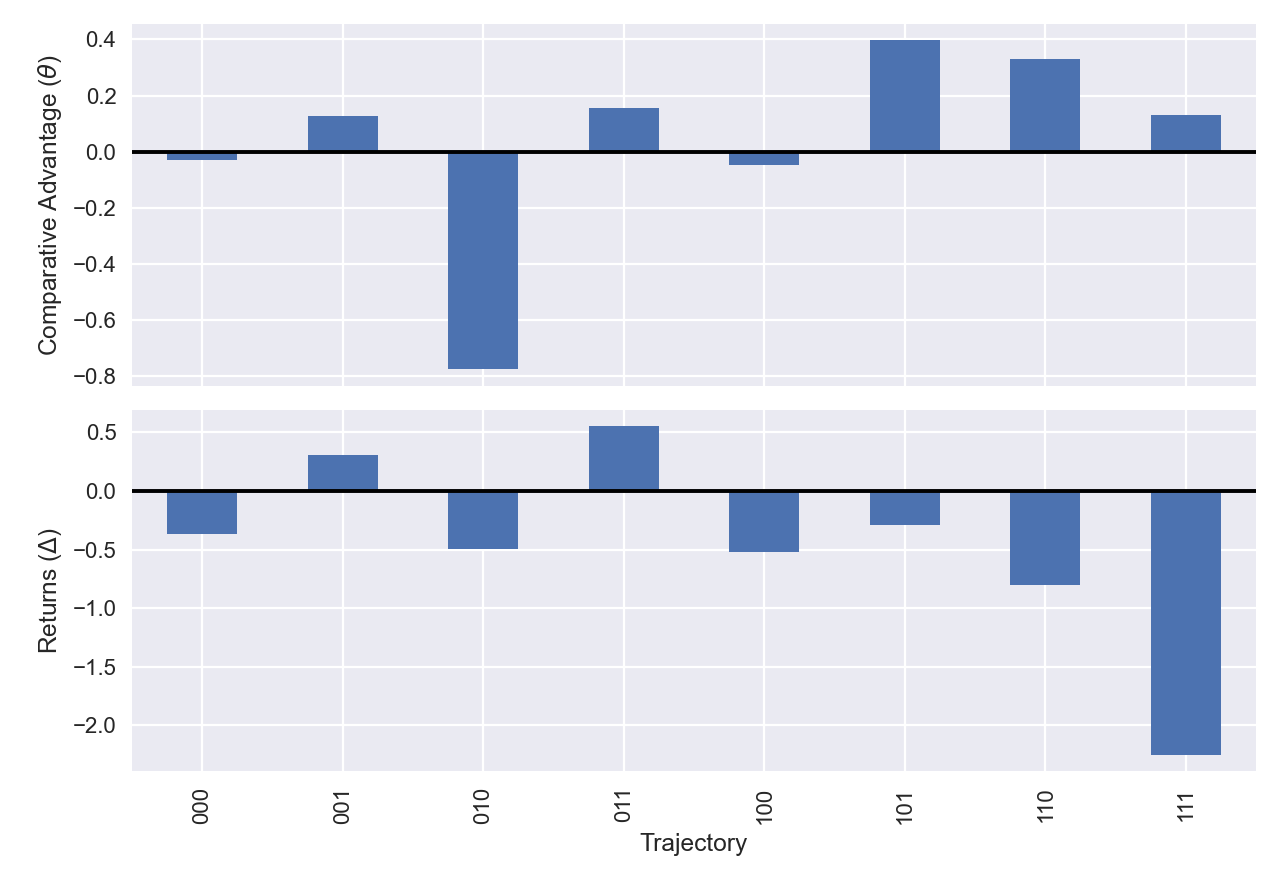
\includegraphics[scale=0.7]{results/figures/theta.png}\label{fig:theta_delta_raw}
        \vspace*{-2em}
    \begin{table}[H]
        \centering
        \begin{tabular}{p{0.8\textwidth}} 
            \begin{tablenotes}
                  \small
                  \item Note: Author's calculations using ESS. The figures shows the comparative advantage and the returns to adoption for each adoption trajectory. Dry cropcuts only
            \end{tablenotes}
        \end{tabular}
    \end{table}
\end{figure}

To explore this further, we run a similar regression to calculate the comparative advantage of adopting a certain number of times. This is similar to Eq. \ref{eq:GRC_Suri}, but uses the number of times that a household adopted hybrid maize (here, $NAdopt$), not its trajectory.

\begin{align}
y_{it}&=\sum_{\underline{na}\in\mathcal{NA}\backslash 3}\nu_{\underline{h}}+\Delta_{(0,0,1)}h_{it}+\phi(\nu_{(0,0,1)}-\nu_{(0,0,1)})_{it}1\{NAdopt_{i}=1\}\nonumber\\
&~~~+\left(\nu_{(1,1,1)}+\phi\left(\nu_{(1,1,1)}-\nu_{(0,0,1)}\right)\right)h_{it}1\{NAdopt_{i}=3\} + X_{it}\beta +\varepsilon_{it},\label{eq:GRC_NAdopt}
\end{align}

In this, instead of a set of trajectories, we have a set of the number of times adopted $\mathcal{NA}$. $\nu$ denotes the average yield from adoption $na$ times. We use adopting once as the base. Figure \ref{fig:n_adopt} shows the results of the regression and calculation of comparative advantage. As expected, adopting 0 times leads to negative comparative advantage, but with positive returns to adoption, implying that there is value to adopting to those that have never adopted hybrid maize seed. Adopting once leads to both positive comparative advantage, and positive returns to adoption. However, adopting twice actually leads to negative comparative advantage, and less positive returns. Adopting all three times leads to positive comparative advantage, but negative returns.

\begin{figure}
    \centering
    \caption{Aggregation Results: Comparative Advantage and Returns by the Number of Times Adopted (Dry Cropcuts)}
    \label{fig:n_adopt}
    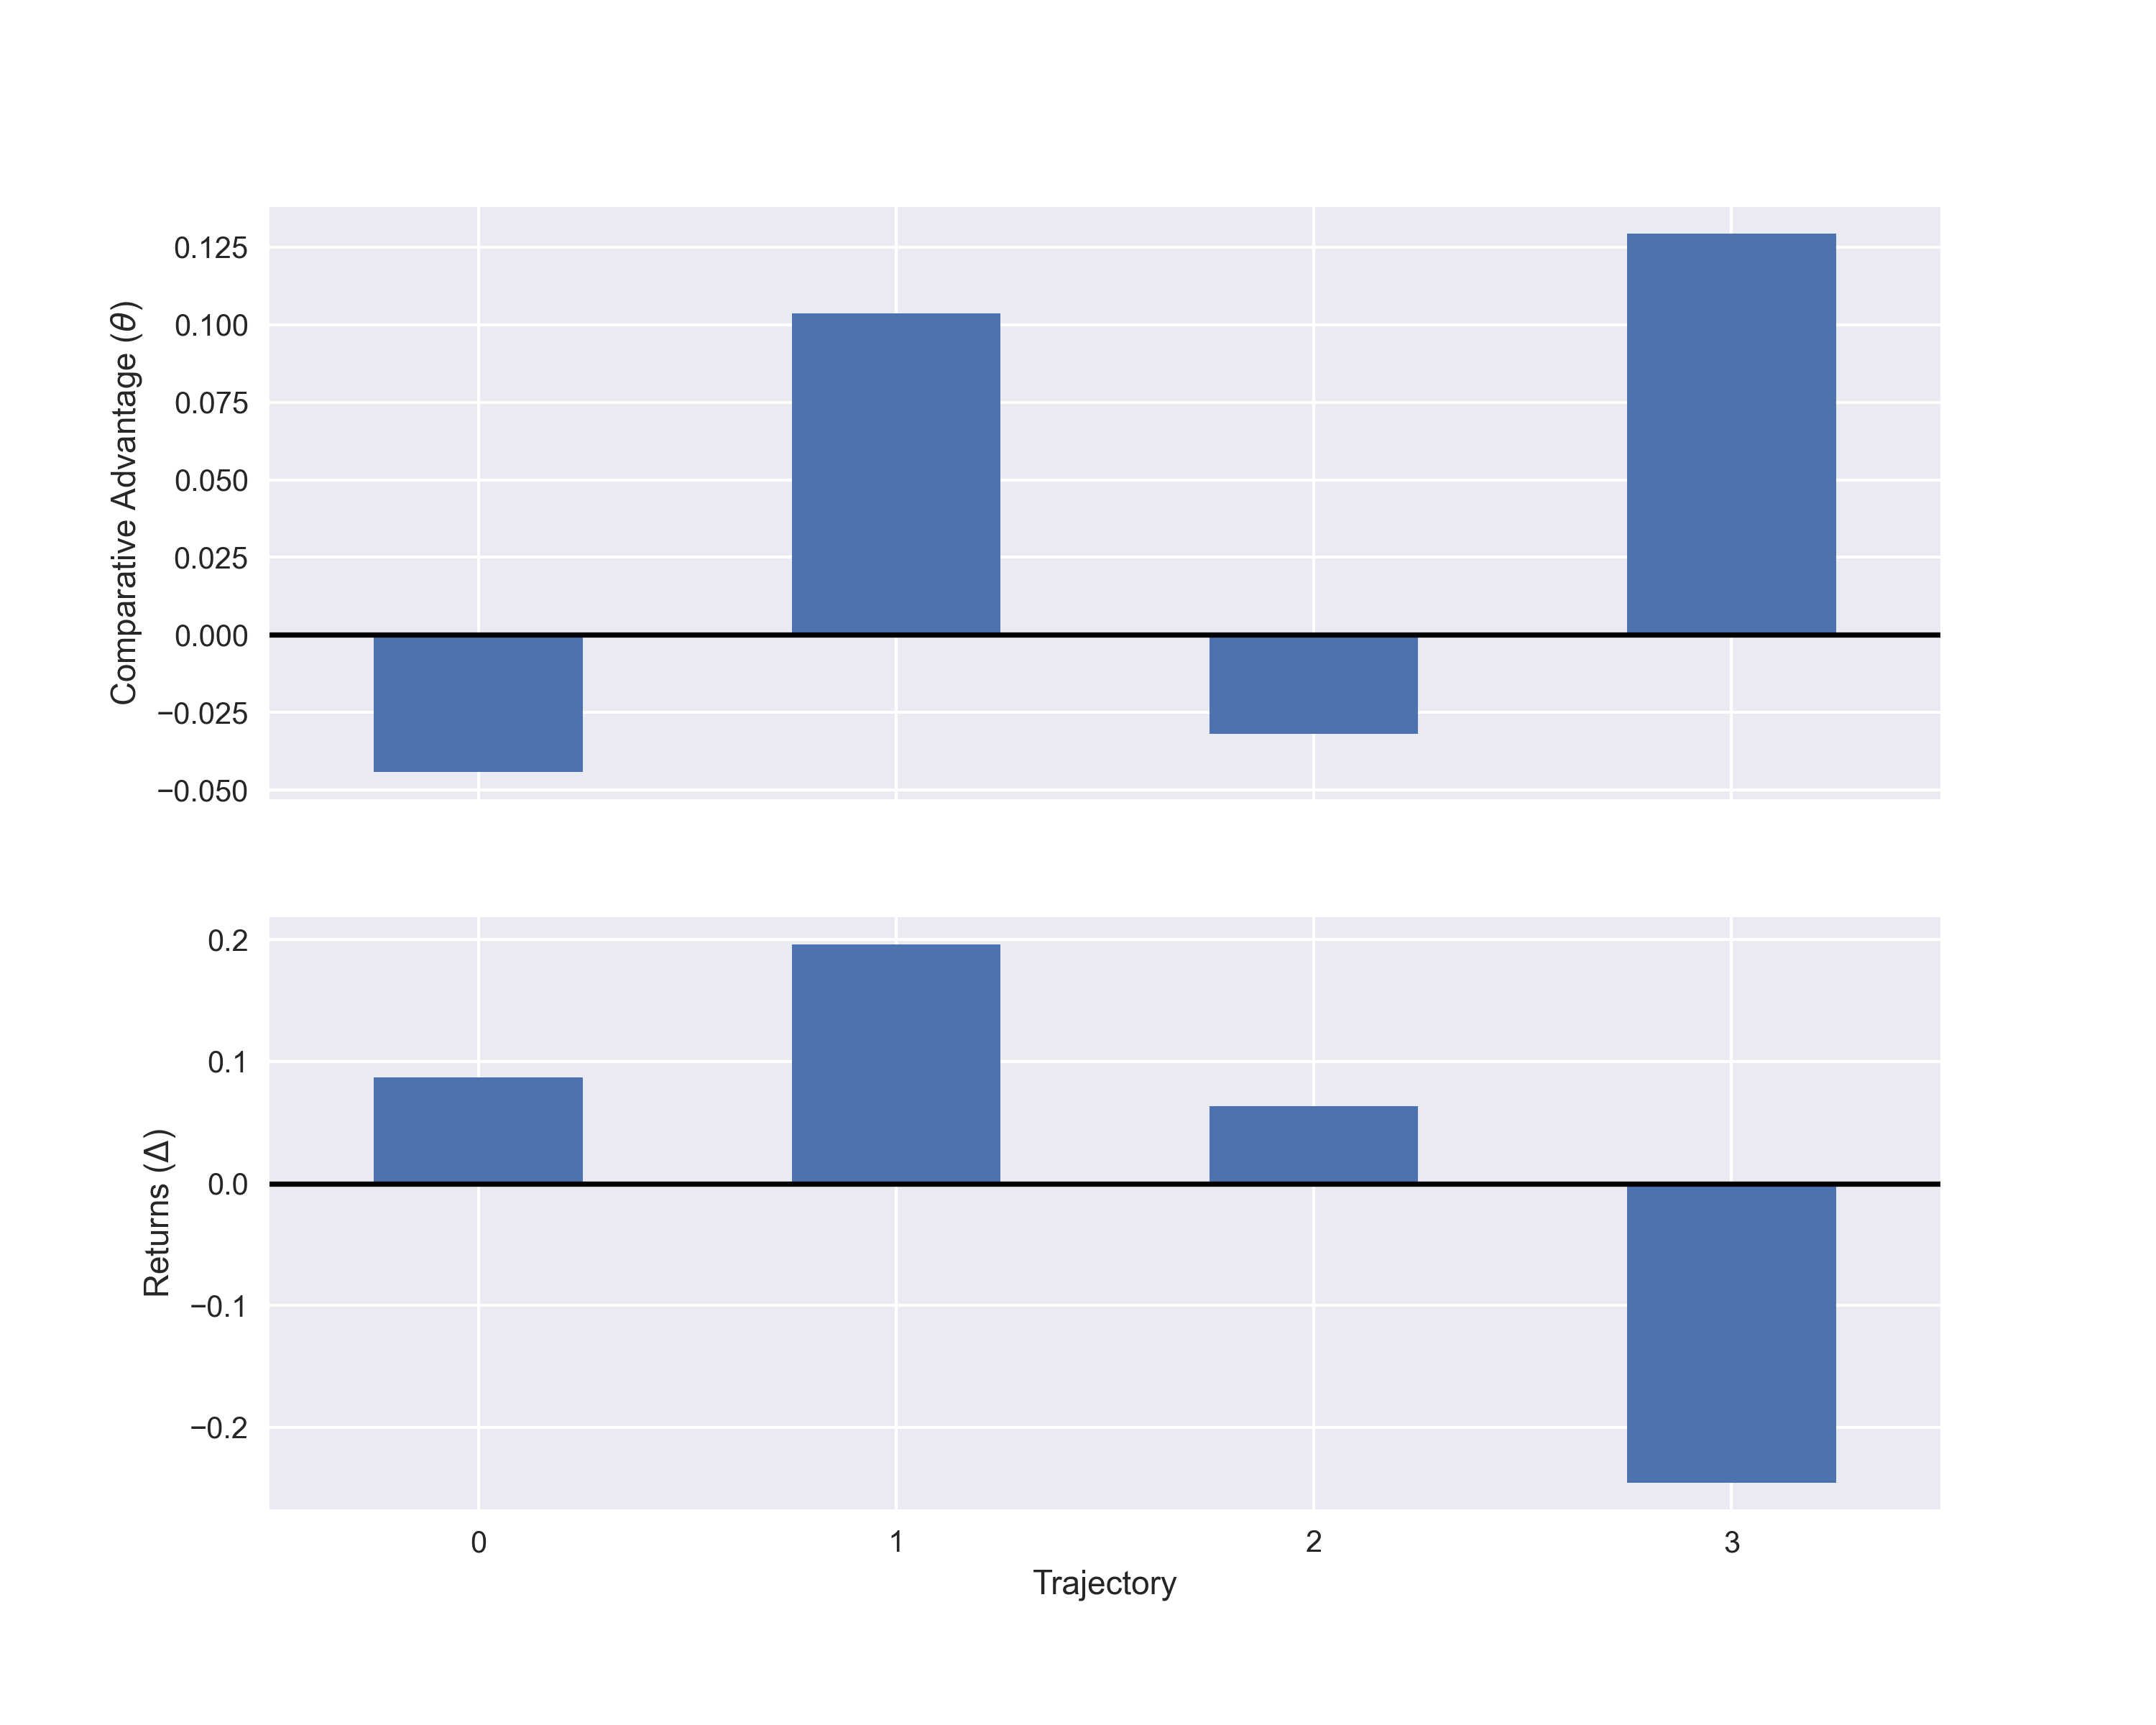
\includegraphics[scale=0.75]{results/figures/num_adoption.png}
    \vspace*{-2em}
    \begin{table}[H]
        \centering
        \begin{tabular}{p{0.75\textwidth}} 
            \begin{tablenotes}
                  \small
                  \item Note: Author's calculations using ESS. The figures shows the aggregate impact from Table \ref{tbl:unres} using the number of time a person adopted as the basis for the aggregation.
            \end{tablenotes}
        \end{tabular}
    \end{table}
\end{figure}



\subsection{Endogenous Switching Regression}

To complement the results of the GRC model, we present the Endogenous Switching Regression results. We first examine a self-reported definition of an improved variety to validate the results from the GRC model. As before, we consider a looser definition of improved seeds, which includes new seeds but also second-generation and recycled (SR1), and a more strict definition, which includes only new varieties (SR2). Table \ref{tab:switch1} shows the results of the Switching regression using both definitions, and using self-reported and cropcut yields. We see that regardless of the definition of improved seed, yields measurement form and types of controls included, the results consistently show that the ATT is negative and the ATU is positive, meaning that farmers that adopted a self-reported improved seed would've been better off not adopting, and farmers that did not adopt a self-reported improved seed would've been better off adopting. 

\begin{table}[H]
\centering
\hspace*{-1.2cm}
\begin{threeparttable}
\caption{Effects on yields (log) from adopting improved maize varieties (self-reported)}
\label{tab:switch1}
\begin{tabular}{l cccccc}
\hline
\hline
            &Adopters yields&Non-adopters yields&         ATE&          SE&     p-value\\
\hline
\textit{SR1, SR yields}&            &            &            &            &            \\
ATT         &        7.30&        9.07&       -1.76&       0.011&      0.0000\\
%
%
%
ATU         &        9.06&        6.87&        2.19&       0.024&      0.0000\\
%
%
%
\textit{SR1, cropcut yields}&            &            &            &            &            \\
ATT         &        7.57&        7.86&       -0.30&       0.017&      0.0000\\
%
%
%
ATU         &        8.89&        7.11&        1.78&       0.039&      0.0000\\
%
%
%
\textit{SR1, SR yields, full set of controls}&            &            &            &            &            \\
ATT         &        7.28&        7.82&       -0.54&       0.019&      0.0000\\
%
%
%
ATU         &        9.65&        6.85&        2.80&       0.100&      0.0000\\
%
%
%
\textit{SR1, cropcut yields, full set of controls}&            &            &            &            &            \\
ATT         &        7.56&        7.61&      -0.049&       0.019&      0.0087\\
%
%
%
ATU         &        9.24&        7.11&        2.13&       0.085&      0.0000\\
%
%
%
\textit{SR2, SR yields}&            &            &            &            &            \\
ATT         &        7.30&        7.85&       -0.55&       0.020&      0.0000\\
%
%
%
ATU         &        9.63&        6.88&        2.75&       0.101&      0.0000\\
%
%
%
\textit{SR2, cropcut yields}&            &            &            &            &            \\
ATT         &        7.61&        7.62&      -0.013&       0.019&        0.47\\
%
%
%
ATU         &        9.35&        7.14&        2.21&       0.091&    1.6e-130\\
\hline
\hline
\end{tabular}
\begin{tablenotes}
\footnotesize
\item{Note: Full set of controls include: parcel size (in HA), household labor, hired labor, fertilizer costs, other input costs irrigation (dummy), mechanization (dummy), organic fertilizer (dummy). Instruments for the adoption equation include: years of education of hh head, age of hh head, female head, land title, asset index, seed costs. Results for SR2 include full set of controls. SR1=1 if New, 2nd gen or recycled,=0 if Traditional; SR2=1 if New, =0 2nd gen, recycled or traditional}
\end{tablenotes}
\end{threeparttable}
\end{table}


To better understand the above puzzling results, we explore similar yield estimations using the different definitions of improved seeds from the DNA fingerprinting. We run similar switching regressions using different thresholds of DNA purity (70, 90 and 95\% purity), for hybrid seeds (compared with open-pollinated varieties), and for Drought-tolerant maize (DTMZ). Table \ref{tab:switch2} shows the results. 

Given that all the plots sampled for DNA fingerprinting showed a purity percent of 70\% or higher, we need a counter-factual to compare these purity thresholds with non-adopters. We therefore consider as non-adopters those that self-reported using a traditional variety. We are aware that given the universality of improved varieties with a 70\% threshold or higher and given the high rates of miss-classification, the control group for a 70\% threshold is likely to be contaminated with a high share of false-positives. But we also know the results are biased downwards and that the control group for higher shares of purity will be less contaminated, which provides an interesting comparison. 

Table \ref{tab:switch2} shows that the estimations for purity thresholds of 70 and 90\% show similar patterns as before: non-adopters would've been better off adopting and adopters would've been better off not adopting. But when improved seeds with a purity of 95\% or higher are compared with self-reported traditional varieties or lower purity than 95\%, the ATT becomes positive and the ATU is still positive but significantly decreases (and it is even negative when self-reported yields are used). Farmers that adopted a variety with a 95\% purity or greater had significantly greater yields than if they had not adopted, considering that this is even a lower boundary. 

We get similar results for DTMZ. Farmers that adopted DTMZ (as tracked by the DNA germplasm) did obtain greater yields than if they had not adopted. Again, this result may be biased downwards because of possible false-positives among the control group. The results for the comparison between hybrid and open-pollinated varieties are not significant (when using self-reported yields).

\begin{table}[H]
\centering
\hspace*{-1.2cm}
\begin{threeparttable}
\caption{Effects on yields (log) from adopting improved maize varieties (DNA fingerprinting)}
\label{tab:switch2}
\begin{tabular}{l cccccc}
\hline
\hline
            &Adopters yields&Non-adopters yields&         ATE&          SE&     p-value\\
\hline
\textit{DNA 70, SR yields}&            &            &            &            &            \\
ATT         &        7.17&        7.31&       -0.14&       0.026&      0.0000\\
%
%
%
ATU         &        8.76&        6.76&        2.00&       0.036&      0.0000\\
%
%
%
\textit{DNA 70, cropcut yields}&            &            &            &            &            \\
ATT         &        7.28&        8.48&       -1.21&       0.041&      0.0000\\
%
%
%
ATU         &        8.55&        7.27&        1.28&       0.042&      0.0000\\
%
%
%
\textit{DNA 90, SR yields}&            &            &            &            &            \\
ATT         &        7.18&        9.07&       -1.90&       0.023&      0.0000\\
%
%
%
ATU         &        7.01&        6.80&        0.21&       0.022&      0.0000\\
%
%
%
\textit{DNA 90, cropcut yields}&            &            &            &            &            \\
ATT         &        7.30&        8.72&       -1.43&       0.028&      0.0000\\
%
%
%
ATU         &        9.32&        7.24&        2.09&       0.034&      0.0000\\
%
%
%
\textit{DNA 95, SR yields}&            &            &            &            &            \\
ATT         &        7.30&        7.08&        0.22&       0.036&      0.0000\\
%
%
%
ATU         &        6.87&        6.86&       0.018&       0.029&      0.5496\\
%
%
%
\textit{DNA 95, cropcut yields}&            &            &            &            &            \\
ATT         &        7.52&        7.39&        0.13&       0.018&      0.0000\\
%
%
%
ATU         &        7.38&        7.12&        0.26&       0.024&      0.0000\\
%
%
%
\textit{HYB, SR yields}&            &            &            &            &            \\
ATT         &        7.28&        7.25&       0.030&       0.028&      0.2892\\
%
%
%
ATU         &        7.06&        6.85&        0.21&       0.028&      0.0000\\
%
%
%
\textit{HYB, cropcut yields}&            &            &            &            &            \\
ATT         &        7.51&        7.55&      -0.038&       0.017&      0.0289\\
%
%
%
ATU         &        7.58&        7.03&        0.55&       0.021&      0.0000\\
%
%
%
\textit{DTMZ, SR yields}&            &            &            &            &            \\
ATT         &        7.42&        6.53&        0.89&       0.074&      0.0000\\
%
%
%
ATU         &        7.11&        7.02&       0.089&       0.022&      0.0001\\
%
%
%
\textit{DTMZ, cropcut yields}&            &            &            &            &            \\
ATT         &        7.56&        6.76&        0.81&       0.058&     3.5e-44\\
%
%
%
ATU         &        8.04&        7.27&        0.77&       0.028&    9.4e-167\\
\hline
\hline
\end{tabular}
\begin{tablenotes}
\footnotesize
\item{Note: Full set of controls include: parcel size (in HA), household labor, hired labor, fertilizer costs, other input costs irrigation (dummy), mechanization (dummy), organic fertilizer (dummy). Instruments for the adoption equation include: years of education of hh head, age of hh head, female head, land title, asset index, seed costs. All results include full set of controls. DNA 70, 90 and 95 refer to improved varieties defined by DNA finerprinting with purity levels of 70, 90 and 95\%, respectively. HYB equals 1 for a hybrid variety, 0 for an open-pollinated variety. DTMZ equals 1 for a Drought-tolerant maize variety}
\end{tablenotes}
\end{threeparttable}
\end{table}


To further disaggregate the results, we explore the source of the improved varieties (CGIAR or exotic) and the year of the seed release. We find positive effects for adopters of CGIAR-sourced varieties when using self-reported yields. The results seem to be contradictory when using cropcut yields, but we should consider these are different samples, as cropcuts were obtained in a subsample of plots. Exotic-sourced varieties also show positive yield effects for adopters; and a negative ATU, meaning non-adopters are also better off not adopting. Newly released-seed varieties do consistently show positive ATT, when using both self-reported and cropcut yields. 

\begin{table}[H]
\centering
\resizebox{0.8\textwidth}{!}{
\hspace*{-1.2cm}
\begin{threeparttable}
\caption{Effects on yields (log) from adopting improved maize varieties (DNA fingerprinting)}
\label{tab:switch3}
\begin{tabular}{l cccccc}
\hline
\hline
            &Adopters yields&Non-adopters yields&         ATE&          SE&     p-value\\
\hline
\textit{CGIAR source, SR yields}&            &            &            &            &            \\
ATT         &        7.13&        6.71&        0.43&       0.033&      0.0000\\
%
%
%
ATU         &        9.19&        6.89&        2.31&       0.018&      0.0000\\
%
%
%
\textit{CGIAR source, cropcut yields}&            &            &            &            &            \\
ATT         &        7.23&        8.98&       -1.75&       0.040&      0.0000\\
%
%
%
ATU         &        7.51&        7.40&        0.11&       0.015&      0.0000\\
%
%
%
\textit{Exotic source, SR yields}&            &            &            &            &            \\
ATT         &        7.13&        6.65&        0.48&       0.022&      0.0000\\
%
%
%
ATU         &        6.83&        6.89&      -0.060&       0.021&      0.0047\\
%
%
%
\textit{Exotic source, cropcut yields}&            &            &            &            &            \\
ATT         &        7.28&        7.18&       0.098&       0.032&      0.0023\\
%
%
%
ATU         &        6.73&        7.33&       -0.60&       0.021&      0.0000\\
%
%
%
\textit{Year 2000+, SR yields}&            &            &            &            &            \\
ATT         &        7.26&        5.55&        1.71&       0.046&      0.0000\\
%
%
%
ATU         &        8.87&        6.93&        1.94&       0.041&      0.0000\\
%
%
%
\textit{Year 2000+, cropcut yields}&            &            &            &            &            \\
ATT         &        7.55&        7.27&        0.28&       0.024&      0.0000\\
%
%
%
ATU         &        8.52&        7.25&        1.27&       0.027&      0.0000\\
%
%
%
\textit{Year 2010+, SR yields}&            &            &            &            &            \\
ATT         &        7.44&        6.92&        0.53&       0.039&      0.0000\\
%
%
%
ATU         &        8.98&        6.91&        2.07&       0.056&      0.0000\\
%
%
%
\textit{Year 2010+, cropcut yields}&            &            &            &            &            \\
ATT         &        7.57&        6.97&        0.60&       0.035&     8.6e-65\\
%
%
%
ATU         &        8.72&        7.25&        1.47&       0.019&           0\\
\hline
\hline
\end{tabular}
\begin{tablenotes}[flushleft]
\footnotesize
\item{Note: Full set of controls include: parcel size (in HA), household labor, hired labor, fertilizer costs, other input costs irrigation (dummy), mechanization (dummy), organic fertilizer (dummy). Instruments for the adoption equation include: years of education of hh head, age of hh head, female head, land title, asset index, seed costs. All results include full set of controls. }
\end{tablenotes}
\end{threeparttable}
}
\end{table}


\subsection{Misclassification-Robust GRC}

The previous results highlight the fact that the definition of hybrid matters. Even when households think they are not adopting hybrid maize seed, there is such a large amount of hybrid seed that has been introduced over the years in Ethiopia that farmers may be misclassifying their seed and taking part in sub-optimal growing strategies as a result. For instance, if a farmer thinks they are growing tradition seed, but they are actually growing hybrid seed, then they will tend to have low returns; hybrid seeds ofte require more fertilizer and other inputs to work optimally. If they are cultivated like traditional seeds, then their performance may end up being worse.

Misclassification of seed is not just a problem in Ethiopia. Countries have been subsidizing inputs and seed for decades and many countries might have the same challenges. In this section, we will introduce a misclassification-robust approach to the GRC method that will allow us to take misclassification into account when calculating comparative advantage. The results from the previous section highlight that there are many definitions to hybrid seed and the fourth wave of the ESS includes DNA fingerprinting. This gives us the ability to validate how often a hybrid seed is actually used when a farmers self-reports adopting hybrid seed. The methodology in this section builds on work that was done in \cite{michuda2021three}, which used confusion matrices from machine learning algorithms as a way to estimate an causal effect that was robust to misclassification. Although, the ESS data does not have results from machine learning algorithms, we can construct a confusion matrix based on the DNA fingerprinting data in the fourth wave and apply it to the previous three waves.

\begin{table}[]
    \begin{subtable}{.5\linewidth}
      \centering
        \caption{Hybrid DNA Purity $>$ 95\% \label{tab:a}}
        \begin{tabular}{lll}
        \toprule
         & 0 & 1 \\
        \midrule
        0 & 0.863 & 0.137 \\
        1 & 0.296 & 0.704 \\
        \bottomrule
        \end{tabular}
        \vspace{1cm}
    \end{subtable}%
    \begin{subtable}{.5\linewidth}
      \centering
        \caption{DNA Fingerprinting for Drought-Tolerant Maize \label{tab:b}}
        \begin{tabular}{lll}
        \toprule
         & 0 & 1 \\
        \midrule
        0 & 0.971 & 0.029 \\
        1 & 0.868 & 0.132 \\
        \bottomrule
        \end{tabular}
        \vspace{1cm}
    \end{subtable} 
    \begin{subtable}{\linewidth}
        \centering
        \caption{DNA Fingerprinting of Seed Released after 2010 \label{tab:c}}
        \begin{tabular}{lll}
        \toprule
         & 0 & 1 \\
        \midrule
        0 & 0.859 & 0.141 \\
        1 & 0.628 & 0.372 \\
        \bottomrule
        \end{tabular}
    \end{subtable}
    \caption{Misclassification Tables for Farmers' Adoption of Hybrid Seed \label{tab:misclassification}}
    \begin{tablenotes}
    \footnotesize
    \item{Note: Table shows three different definitions for misclassifying adoption of hybrid maize. A 0(1)-row denotes that a farmer self-reported using traditional(hybrid) seed. A 0(1)-column is whether the seed was in fact traditional(hybrid). All definitions calculated from ESS data. Sub-table \ref{tab:a} shows the percentage that farmers self-reported using hybrid seed when that seed was at least 95\% pure. Sub-table \ref{tab:b} shows the same table but for whether the seed was drought-tolerant maize seed. Sub-table \ref{tab:c} shows the same table but for hybrid seed released after 2010.}
    \end{tablenotes}
\end{table}

Table \ref{tab:misclassification} shows a table of different hybrid seed definitions and the percentage of times that a farmer self-reported traditional or hybrid seed, and whether they in fact were using traditional or hybrid seed, based on the DNA fingerprinting data. You can see from Sub-table \ref{tab:a} that around 86\% of farmers actually use traditional seed when they self-report using traditional seed, and around 70\% of the time, farmers use hybrid seed of at least 95\% purity when they self-report using hybrid. There are in fact instances where farmers, however, misclassify their self-reports. For instance, in sub-table \ref{tab:b}, a farmer that self-reports using drought-tolerant maize, only in fact uses drought-tolerant maize 13\% of the time. There are similarly large misclassifications for seed released after 2010. The previous section highlighted that different definition of maize could actually lead to vastly different treatment impacts from seed adoption. 

In order to apply these misclassification probabilities to the previous three waves, we made assumptions about the nature of misclassification: that the rate of misclassification is constant across time and exhibits no dynamic behavior. Although these are strong assumptions, they come from the limitations of the data; the fourth wave of the ESS was the first to include DNA fingerprinting, and so was the first where a table like the one in Table \ref{tab:misclassification} could be calculated. Let $p_{ij}$ be the $i,j$th cell of a misclassification table as in Table \ref{tab:misclassification}. Suppose that we construct the probability of being in a true trajectory $h = (i,j,k)$, intersected with being in a reported trajectory $\hat{h} = (\hat{i},\hat{j}, \hat{k})$ as:

\begin{equation}
\label{eq:misclass}
P(h = (i,j,k) , \hat{h} = (\hat{i},\hat{j}, \hat{k})) = p_{i, \hat{i}}\cdot p_{j, \hat{j}}\cdot p_{k, \hat{k}}
\end{equation}

We can use Eq. \ref{eq:misclass} to construct the joint distribution, $f(h, \hat{h})$ for each trajectory in the sample. Since we had the most confidence in the data from Table \ref{tab:a}, we decided to use it for the main body of the paper. 

\section{Conclusion}\label{sec:conclusion}

% - Why do we see that increasing purity leads to positive ATE
% - may be due to improved seed being more effective, but doesnt tell the whole story
% - barrier to purchasing the seed and associated inputs for poorer households, leading to reuse of seeds and being less effective

Our results showcase the challenges of identifying the returns to technology adoption when adoption is not promoted by a randomized control trial and when the characteristics of the technology (genetic purity) are not easily observed. We show that in the case of Ethiopia, the return to adoption of improved seed varieties appears to be negative, a result that we attempt to further understand by relying on seeds' DNA fingerprinting, obtained from the last round of the ESS. Accounting for the decay of the purity of the genetic material, its source and years upon release, reveals that those farmers that rely on newly bred improved varieties do show positive returns to adoption. Even without explicit DNA fingerprinting evidence, the GRC could show this trend with the comparative advantage results; returns are harmful to those with a high comparative advantage to adopt, but these returns are less negative with time. We speculate that this is due to the fact that new and more genetically pure hybrids are introduced giving those that adopt higher yields than before.

But the fact that newly bred hybrids that adapted to local conditions outperform local varieties and older-generation improved seeds is not surprising given the large investments devoted to improve seed performance and the speed at which new high-yielding varieties are being developed. The results from the Group Random Coefficient model highlights how the fact that we imperfectly observe the use of newly improved seeds and the degree of mis-classification between self-reported improved seeds and bred hybrids may partially explain why we do not see self-reported improved varieties grant positive returns to adoption. Reconciling these findings with the results from the Endogenous Switching Regression, we hypothesize that the negative returns to adoption mask a large heterogeneity in the returns to adoption. The switching results show that the positive returns to adoption only appear for those farmers using newly bred hybrid seeds provided directly by distributors. 

This result buttresses the fact that a large share of farmers are not able to obtain the promised greater yields from using hybrid varieties. This may be partially driven by the low-purchasing rates of newly bred varieties, but also by the under-use of critical inputs needed for the successful performance of hybrid seeds, such as fertilizers and irrigation, especially in drought-prone areas. More research is required in order to understand the barriers to adoption and input use. Such barriers may be crucial for households with less resources, which might be more likely to reuse improved seeds for many generations or buy older generations from other farmers at a cheaper price. The fact that all the sampled plots chosen for DNA fingerprinting showed purity percentages of 70 percent or higher is indicative that this might be the case, given the widespread dilution of improved genetic material. Such dispersion of improved genetic material also poses a challenge for the proper identification of the returns to adoption as it confounds the potential benefits of locally adapted hybrids, but also the benefits of traditional local varieties that may be better suited for certain agro-ecological conditions and for contexts of low-input use.  

Our findings are in line with prior research. \cite{Bird2020-nt} propose a theoretical model where the authors compare retained local traditional varieties with improved non-locally adapted varieties and locally adapted improved varieties. The authors postulate that while profits of both types of improved varieties increase with fertilizer application, profits of traditional varieties would decrease with fertilizer application, implying the existence of a threshold of fertilizer application below which it is more profitable to keep using traditional varieties. Non-locally adapted varieties are less profitable without complementary fertilizer application. Depending on how responsive to fertilizer both improved varieties are and on the costs of seeds, there may be a threshold of fertilizer application below which it is more profitable to use the locally adapted variety than the improved non-adapted one. \par

It is possible that similar dynamics explain the patterns showcased in our results. The evidence is consistent in that newly bred varieties do offer higher performance than traditional varieties, but such higher-yielding effects diminish over time, as newer generations of the improved seeds continue to be used. In contrast, traditional local varieties are well-adapted to the local agro-ecological conditions, and their reproduction over multiple generations shows consistent yields, assuming normal weather conditions. Depending on the specific improved varieties and the speed at which high-yielding effects diminish over time, there may be a threshold in time above which it may be more profitable to use a traditional variety than an improved one that has been around for too many generations. After such a threshold is reached, because improved varieties are more dependent on external inputs, the costs of the older-generation improved seeds, together with the costs of fertilizers and other inputs may not compensate the yield returns of an older-improved variety. \par

Our results have far-reaching policy implications. The adoption and impact of genetically improved seeds are inherently heterogeneous. Our methodology incorporates this from the outset. Our findings highlight the wide distribution of the yield returns to adoption, partially explained by the low purchase of newly bred hybrids and the high dispersion of diluted improved genetic material over time. This points to the need for making policies oriented towards increasing the adoption of improved seeds and yields more inclusive, aiming at ensuring that improved varieties are not only available to purchase locally but also affordably. It is important to consider that improved varieties should also be locally adapted to specific agro-ecological conditions, such that their success is less dependent on external chemical inputs. Our findings also shed light on the need to better understand adaptation strategies when the conditions needed for the successful performance of improved seeds are lacking. These contexts include but are not limited to places subject to high weather variability or where low soil fertility is prevalent due to the use of excessive intensification and chemical input dependence. Resilience-enhancing strategies such as the use of drought-tolerant maize or irrigation use may be critical for such contexts, but their suitability for the heterogeneous pool of farmers needs to be better understood. 


%allowing us to investigate whether synergies between seed adoption and water conservation strategies interact; a key component to understanding how investment into such projects translates to economic returns. Moreover, our research informs on not only the adoption but also dis-adoption decisions of technologies as well. In this sense, we provide valuable information to policymakers on how to better target seed marketing or infrastructure to help agricultural households improve their livelihoods






\bibliography{references}


\end{document}